\chapter{The System Development}\label{cap:development}
Na seção de desenvolvimento desta tese, serão apresentadas as etapas de elaboração do sistema proposto, bem como a metodologia aplicada e os resultados obtidos ao longo do processo. A discussão e análise dos dados coletados permitirão avaliar a eficácia do sistema implementado, destacando os avanços obtidos na rastreabilidade e gestão dos componentes fabricados, e propondo melhorias e ajustes necessários para aprimorar ainda mais a solução apresentada.

\section{Case Study Scenario}\label{section:caseStudyScenario}

Esta dissertação de mestrado concentra-se no estudo de caso da Mofreitas, uma \acrfull{smes} especializada na produção de mobiliário em madeira. A fabricação dos móveis envolve processos parcialmente manuais e automatizados, empregando maquinário de corte, como fresas, \acrfull{cnc}, nesting e orlagem. Um dos desafios enfrentados pela empresa reside na rastreabilidade dos componentes produzidos, abrangendo aspectos como as peças individuais, o estágio do projeto, os materiais remanescentes após a confecção e os materiais terciários consumidos ao longo do decorrer do projeto. Desse modo, verifica-se uma complexidade tanto na rastreabilidade do projeto quanto na gestão de inventário.

Pra um melhor entendimento do problema, é necessário um entendimento prévio do fluxo de execução das etapas envolvidas. O processo produtivo da carpintaria Mofreita inicia-se com a concepção da solução de mobiliário pelo cliente, que pode apresentar diferentes níveis de detalhamento, desde projetos completos até esboços manuais ou ideias vagas. Para a formalização do projeto, são estabelecidas informações em conjunto com o cliente por meio de reuniões presenciais, troca de e-mails ou chamadas telefônicas, e os detalhes discutidos são registrados no software OneNote\textsuperscript{\textregistered} \cite{onenote}.

Após essa fase, o processo de orçamentação tem início com o suporte de uma planilha desenvolvida no Microsoft Excel \textsuperscript{\textregistered} \cite{excel2023}. Com a aceitação do orçamento pelo cliente, o desenho técnico associado ao projeto é realizado, utilizando o software SolidWorks\textsuperscript{\textregistered} \cite{solidworks}. Durante essa etapa, o cliente é consultado para possíveis ajustes e correções no projeto e no orçamento.

Ao concluir o desenho técnico, os arquivos gerados pelo software \acrshort{cad}, no formato Parasolid, são importados para o software AlphaCAM\textsuperscript{\textregistered} \cite{alphacam}, responsável pela geração dos arquivos necessários para as máquinas de nesting e programação de máquinas de fresar \acrfull{cnc}. No ambiente de trabalho do software \acrfull{cam}, os arquivos são organizados manualmente em pastas internas, de acordo com a espessura das placas de madeira utilizadas no projeto. Em seguida, o processamento por esse programa gera os arquivos base para as máquinas de nesting e CNC, os quais são armazenados em uma pasta compartilhada e identificada com a referência do projeto.

Ademais, estes documentos são empregados na produção de registros intitulados "listas de corte" e "listas de acessórios". Tais listas possibilitam a consulta acerca das características e quantidades individuais de cada componente do projeto em questão, através de referência. Ilustrativamente, a Figura \ref{fig:cutLsitMyCad} apresenta um exemplar dessas mencionadas listas de corte. Este ficheiro, em formato \acrfull{csv}, é gerado automaticamente por um software integrado no ambiente SolidWorks\textsuperscript{\textregistered} por um "add-on" designado por MyCADTools\textsuperscript{\textregistered} \cite{mycadtools} sendo posteriormente utilizado no software S2M CENTER\textsuperscript{\textregistered} \cite{s2mcenter}, para gerar as etiquetas que serão utilizadas para identificar os vários elementos de madeira cortados pelas máquinas \acrshort{cnc}. A Figura \ref{fig:tagExample} apresenta o aspeto de uma dessas etiquetas.


\begin{figure}[h!]
    \centering
    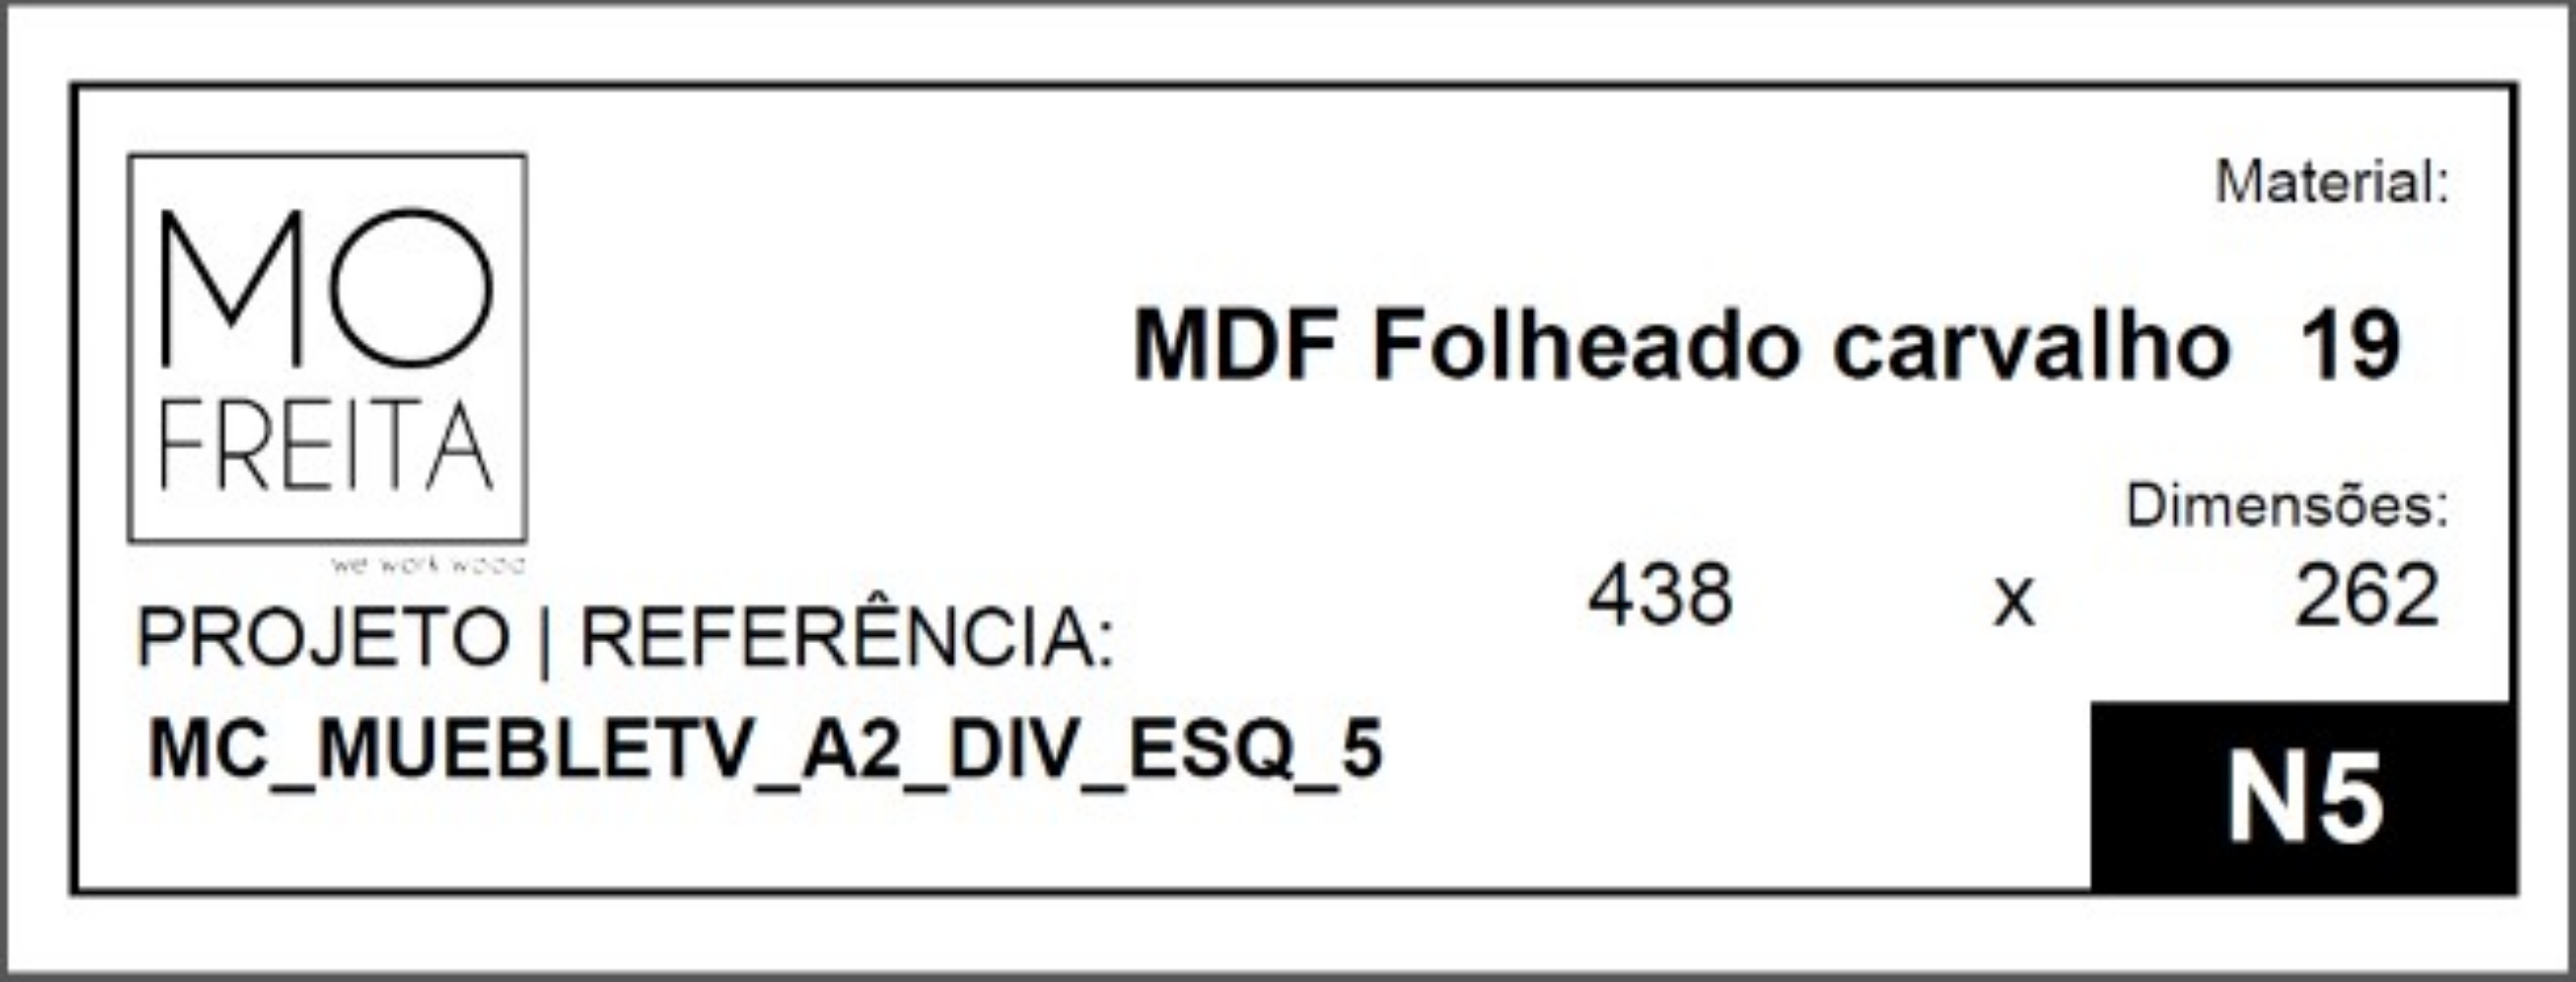
\includegraphics[width=.65\linewidth]{images/Development/chap4/tagExample.png} 
    \caption{This is an example of a tag generated by the S2M CENTER\textsuperscript{\textregistered} software. The aforementioned label contains pertinent information about the wood component used in the manufacture of the furniture. Among this information, the specification of the material, dimensions and the identification denomination stand out, which establishes a correlation with the CAD drawings.}
    \label{fig:tagExample}
\end{figure}

Importa salientar que uma reprodução dessas listas, materializada em papel, é encaminhada para a área de produção. Este documento acompanha todos os componentes cortados de um determinado projeto e serve de guia para os operadores. Proporciona-lhes o conhecimento acerca de quais peças produzir, de qual material se vale, quais operações são executadas e em que sequência. Adicionalmente, estas listas facultam o registro do que já foi processado e do tempo despendido nesse processamento.


Os arquivos produzidos pelo AlphaCAM\textsuperscript{\textregistered}, cruciais para a programação das má-\\quinas de nesting e CNC, são introduzidos no software de controle correspondente a cada maquinário, sendo acionados mediante instruções fornecidas pelos operadores. Tal como mencionado anteriormente, esses arquivos, juntamente com as etiquetas de identificação que devem ser aderidas nas peças após o nesting, estão acessíveis em todos os computadores da área de produção, localizados numa pasta compartilhada em nuvem. Ademais, os operadores têm a possibilidade de consultar e proceder à visualização tridimensional de cada um dos projetos, por meio da abertura dos arquivos gerados no SolidWorks\textsuperscript{\textregistered} utilizando o software de visualização eDrawing\textsuperscript{\textregistered}.


Após a etapa de corte e processamento de cada um dos componentes de madeira inerentes ao projeto, dá-se início ao procedimento de montagem. O propósito desta fase é assegurar que a confecção dos móveis tenha sido realizada em conformidade com as especificações do projeto, permitindo assim a mitigação de erros no local final de entrega, que muitas vezes está a uma distância significativa do local inicial de fabricação.

Esta fase frequentemente requer a utilização de diversos consumíveis, tais como parafusos, buchas e cola, assim como uma gama de ferragens, incluindo dobradiças, puxadores e fechos. No âmbito da gestão de estoques, os consumíveis são adquiridos no armazém por um operador designado, em volume que satisfaça a demanda. Durante este processo, o operador é encarregado de registrar, de forma escrita, a descrição do número de caixas de pregos, parafusos, entre outros itens que foram requisitados.

Quanto às ferragens, a lista deste material, vinculada a um projeto específico, é processada diretamente pelo responsável do armazém. Neste contexto, a totalidade destes itens é segregada em caixas, sendo associada, por meio de referência, ao projeto correspondente.


Após a etapa de montagem, ajuste e inspeção cuidadosa de todos os elementos de mobiliário associados ao projeto, dá-se início à fase de embalagem. Neste estágio crucial, os componentes são acondicionados de maneira segura para garantir a sua integridade durante o transporte. Além disso, são devidamente identificados, não apenas para assegurar a rastreabilidade e facilitar o manuseio durante o trânsito, mas também para auxiliar na montagem correta no local de destino. Esta identificação é de suma importância, pois contém instruções detalhadas e a sequência de montagem, garantindo que a montagem final seja efetuada de acordo com as especificações do projeto e prevenindo o extravio de componentes, o que poderia gerar significativos transtornos logísticos. Este processo de embalagem é meticulosamente planejado e executado, visando não somente a proteção física dos móveis, mas também a otimização do espaço no transporte.




Até o presente momento, foram abordadas as diversas fases do processo produtivo vinculado à fabricação de um componente de mobiliário específico na carpintaria Mofreita. Este trajeto se inicia na proposta de projeto e culmina no produto final, já instalado no local do cliente. Dentre os subprocessos que são indispensáveis para a fluidez e consolidação desta cadeia produtiva, a gestão de estoques é um elemento de destaque.

São identificadas dificuldades primordiais em dois eixos: o primeiro concerne à logística associada aos consumíveis e ferragens e o segundo à rastreabilidade dos resíduos de madeira que surgem da execução das listas de corte. No que tange ao primeiro eixo, emerge a necessidade premente de digitalizar o processo de requisição de consumíveis e ferragens, objetivando evitar o registro manual e favorecer a integração em tempo real dessas informações ao processo de gestão como um todo.

Adicionalmente, a atual administração de dados referentes aos estoques é efetuada mediante uma planilha genérica, o que obstrui o registro automático de informações temporais correlacionadas às entradas e saídas de material, assim como às eventuais flutuações de preço. Portanto, a atualização do software de gestão de estoques é um passo fundamental na direção da modernização do processo produtivo.

A solução proposta deve promover, além do armazenamento de informações pertinentes aos estoques, a possibilidade de análise desses dados. Esta capacidade possibilita a geração de estatísticas que respaldem de maneira mais eficaz o processo de tomada de decisões. Dados como o intervalo de tempo entre pedidos para uma referência específica e os tempos médios de entrega de um fornecedor particular são de suma importância. Dada a singularidade intrínseca a cada projeto, é possível apenas estabelecer uma previsão para o tempo de produção. Tal previsão poderia ser delineada a partir do histórico de projetos anteriores que guardassem similaridade em termos de quantidade de cortes e etapas de montagem requeridas. Nesse sentido, a solução proposta pelo WW4.0 é esperada para registrar esse tipo de informação, associando a cada projeto os tempos requeridos para o processamento de cada um de seus componentes.

No que concerne à cadeia de produção, a maneira como as matérias-primas são incorporadas à linha de produção é a segunda questão que o WW4.0 pretende abordar. Especificamente, o destino dos resíduos de cada projeto e como esses resíduos podem ser automaticamente reintegrados à cadeia é um ponto de interesse. Atualmente, não há atualização automática das informações, na planilha utilizada para controle de estoques, sobre as matérias-primas remanescentes dos diversos processos de corte. As placas de madeira que sobram ao longo da semana de trabalho, e que possuem uma área considerada aproveitável, são reorganizadas manualmente e reintegradas à zona de armazenamento. Seu uso subsequente é realizado pelos operadores, por meio de inspeção visual, visando a um propósito específico. Este método operacional é subótimo, pois resulta em um maior desperdício do que se esses resíduos fossem utilizados em processos de nesting.

Portanto, o objetivo é adotar uma estratégia de rastreamento da matéria-prima remanescente, de forma que ela possa ser automaticamente integrada ao estoque para ser reutilizada de maneira mais eficiente em projetos de fabricação subsequentes. Em particular, para cada resíduo, pretende-se registrar suas dimensões, tipo de material, espessura e localização no chão de fábrica. Além disso, é crucial conhecer, se aplicável, a direção dos veios da madeira. A solução a ser desenvolvida no contexto do WW4.0 deverá permitir a identificação, no chão de fábrica, de cada resíduo, bem como sua integração na lista de estoques com todas as características mencionadas anteriormente. Essas informações deverão ser utilizadas para minimizar ainda mais o desperdício de matéria-prima e tornar todo o processo mais eficiente.




\begin{figure}[h!]
    \centering
    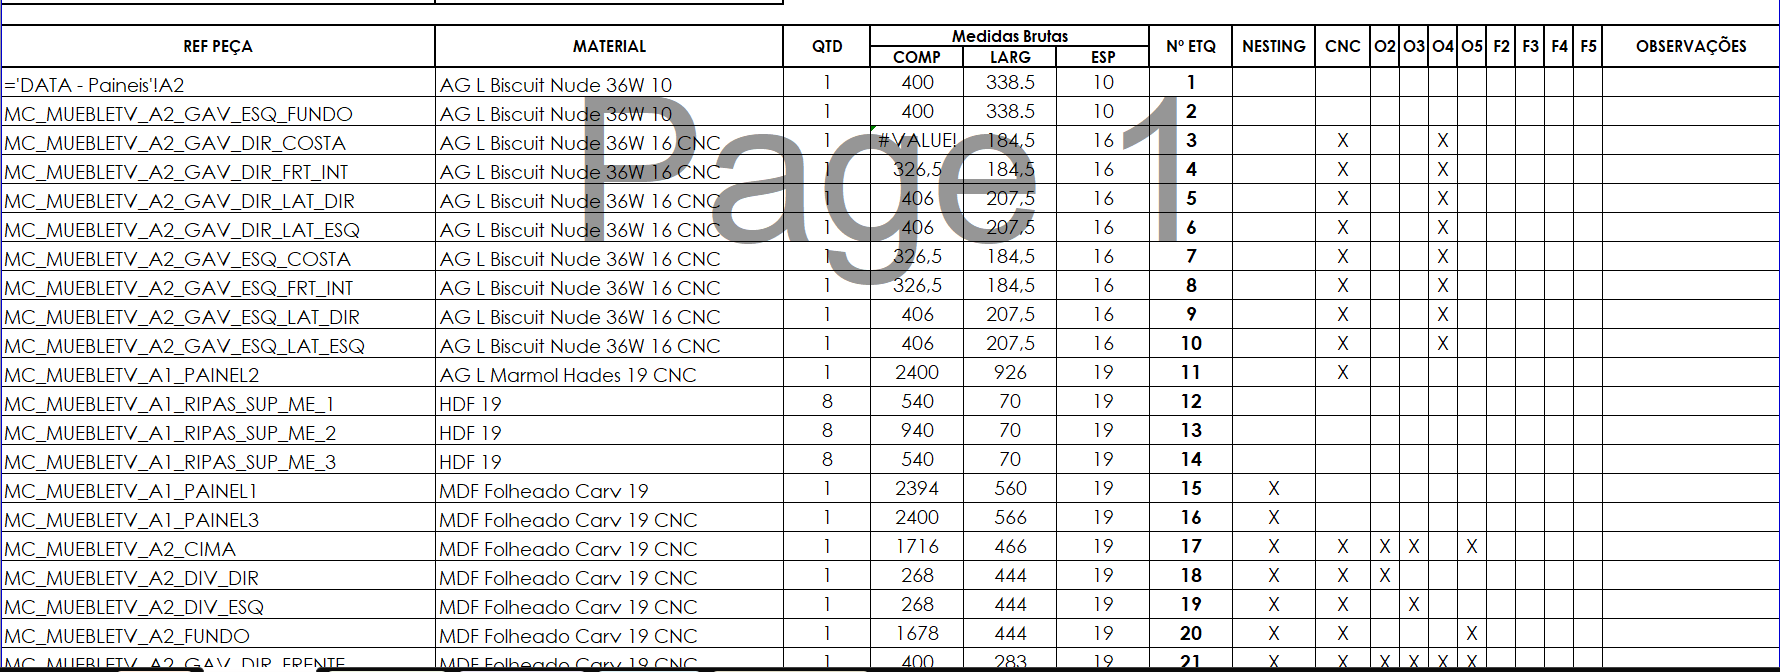
\includegraphics[width=.65\linewidth]{images/Development/chap4/ListaDeCorte.png}
    \caption{Excerpt from a cut list generated by MyCADTools software.}
    \label{fig:cutLsitMyCad}
\end{figure}


Além do mais, essa abordagem apresenta desafios relacionados à padronização e dificulta o rastreamento dos projetos. Diante desse contexto, o propósito primordial desta pesquisa é desenvolver um sistema que viabilize a rastreabilidade dos itens produzidos na fábrica, utilizando informações obtidas das planilhas Excel \textsuperscript{\textregistered} e dos ecrãs localizados na área de produção, que recebem entradas de dados fornecidas pelos usuários.

\begin{figure}[h!]
    \centering
    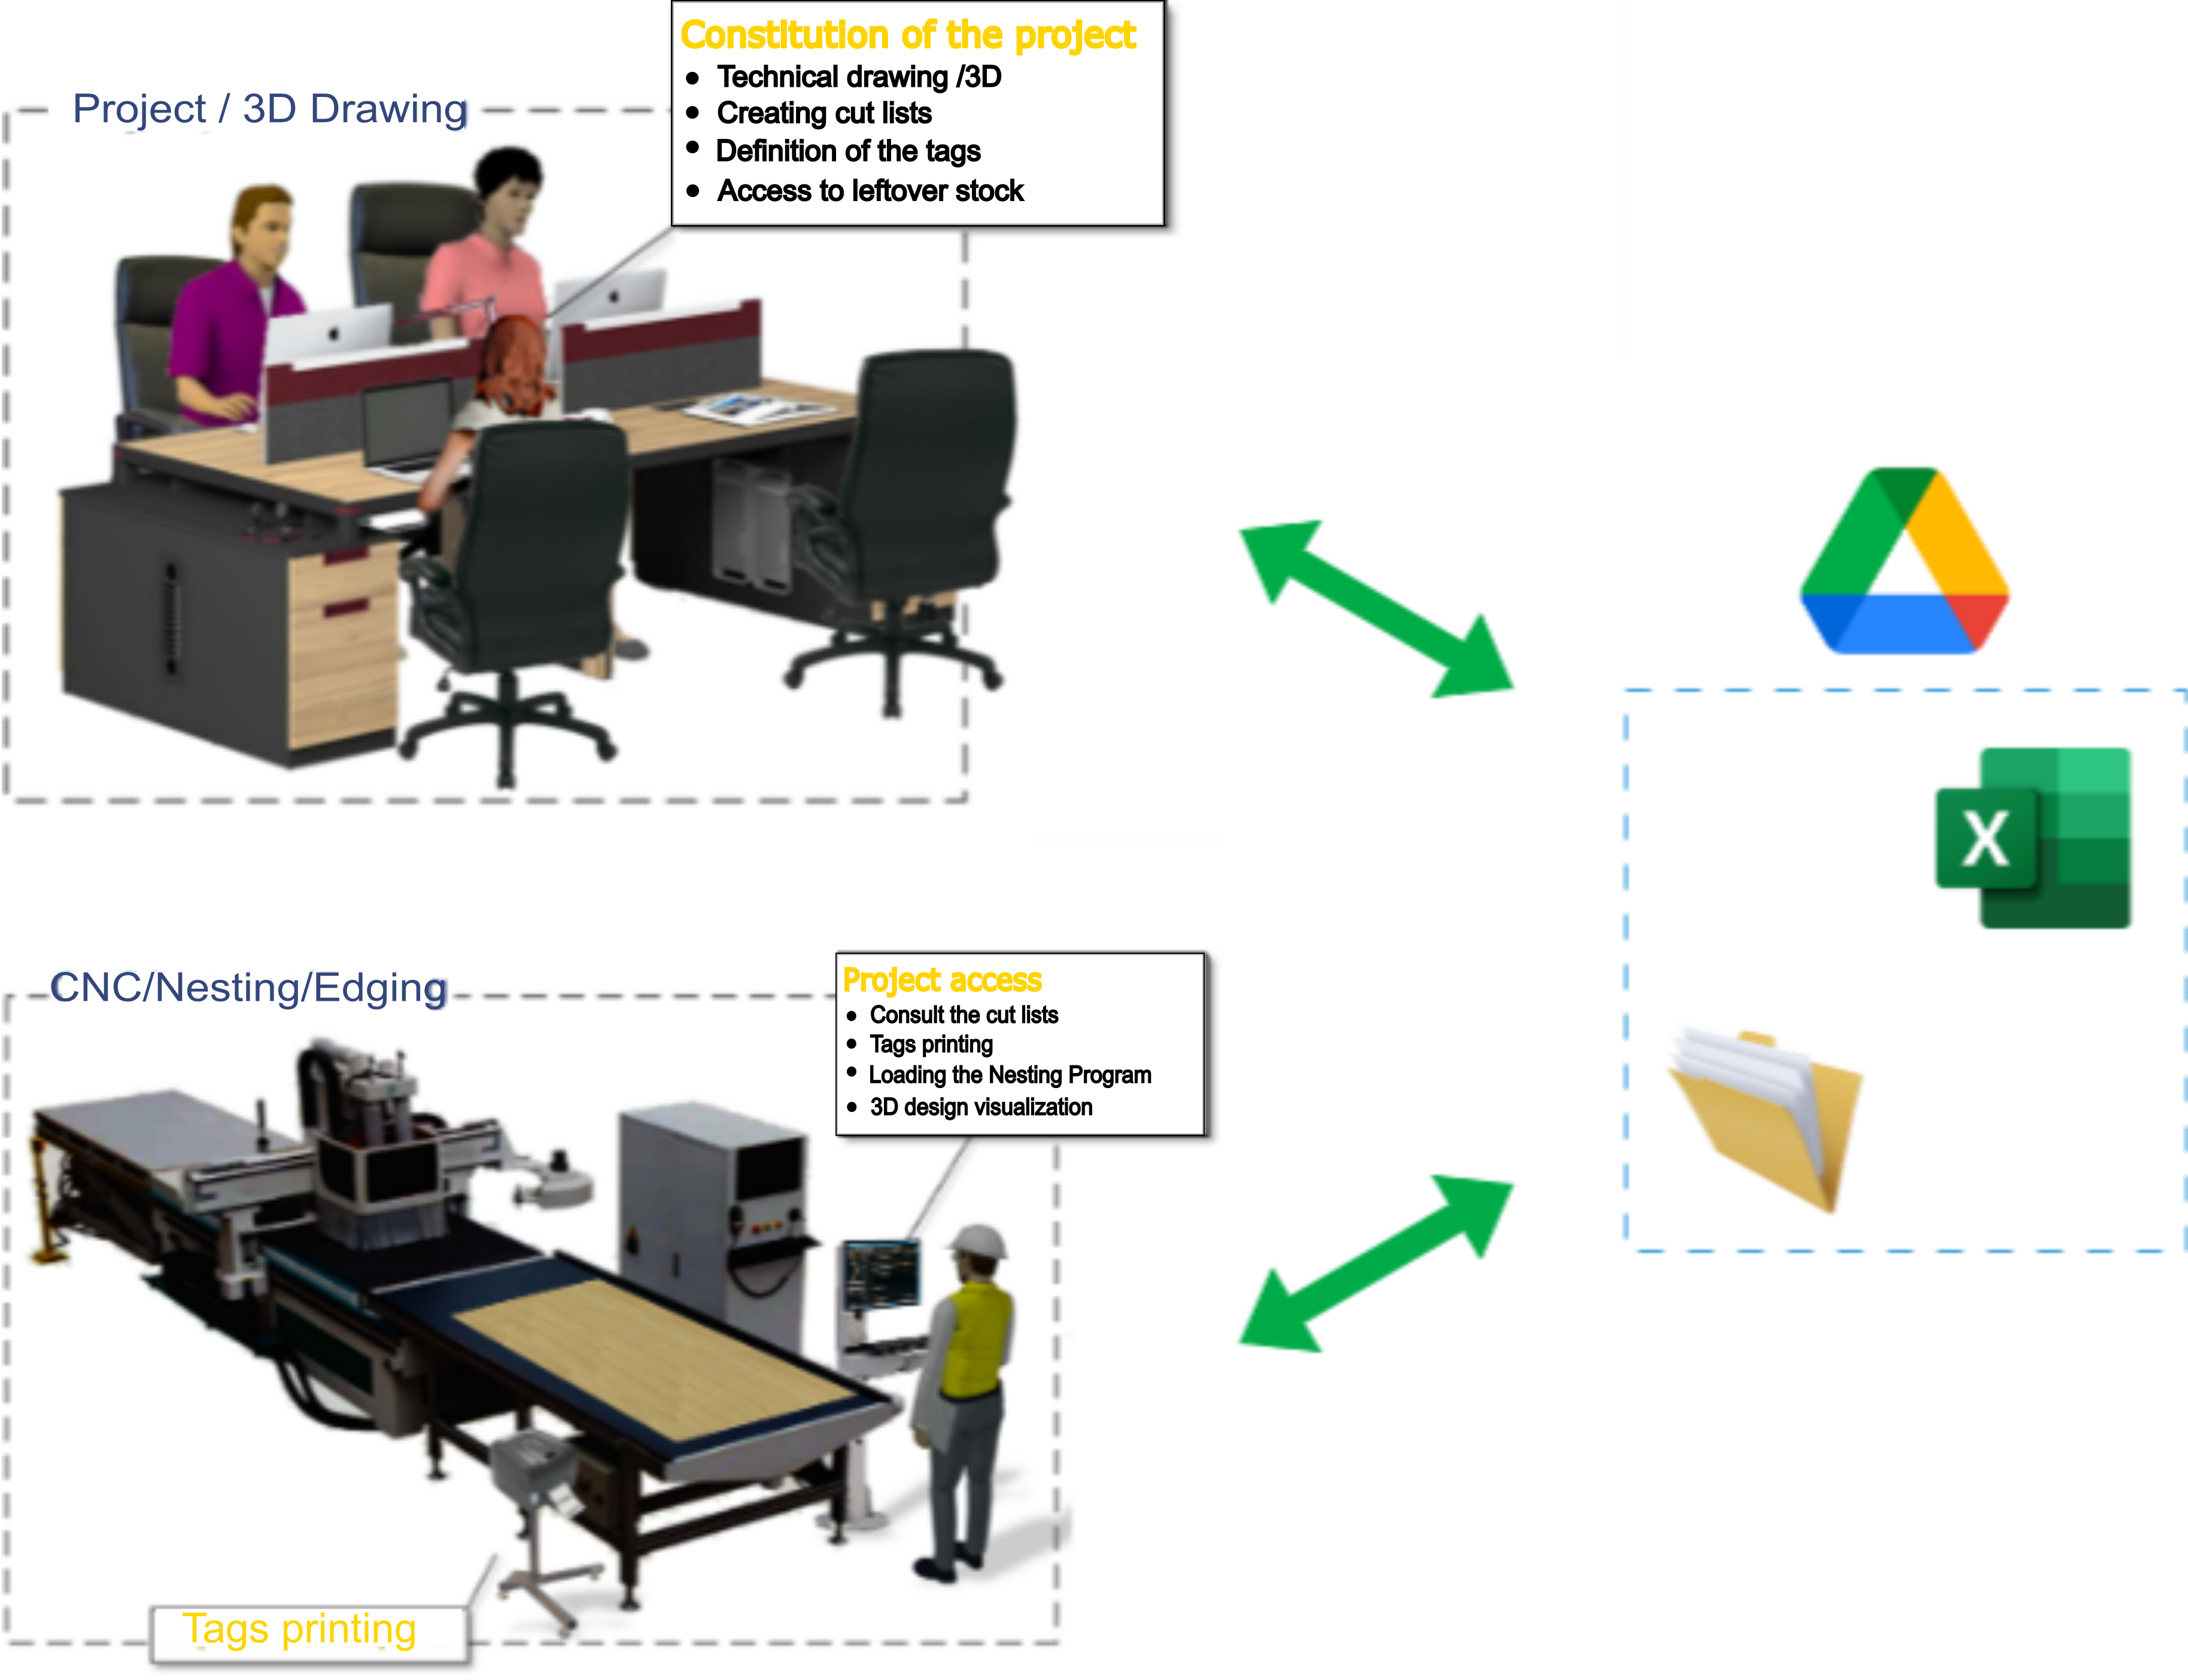
\includegraphics[width=.65\linewidth]{images/Development/chap4/MofreitasCase.png}
    \caption{Graphical representation of how mofreitas initially accessed project information in different locations on the factory facility.}
    \label{fig:dataSharing}
\end{figure}
O arquivo em formato CSV é gerado automaticamente por um software integrado ao ambiente SolidWorks®, denominado MyCADTools®, e posteriormente utilizado no software S2M CENTER®, comercializado pela empresa Cabinet Vision®, para a criação das etiquetas que identificarão os diversos elementos de madeira cortados pelas máquinas CNC. A Figura 6 ilustra a aparência de uma dessas etiquetas.

\begin{figure}[h!]
    \centering
    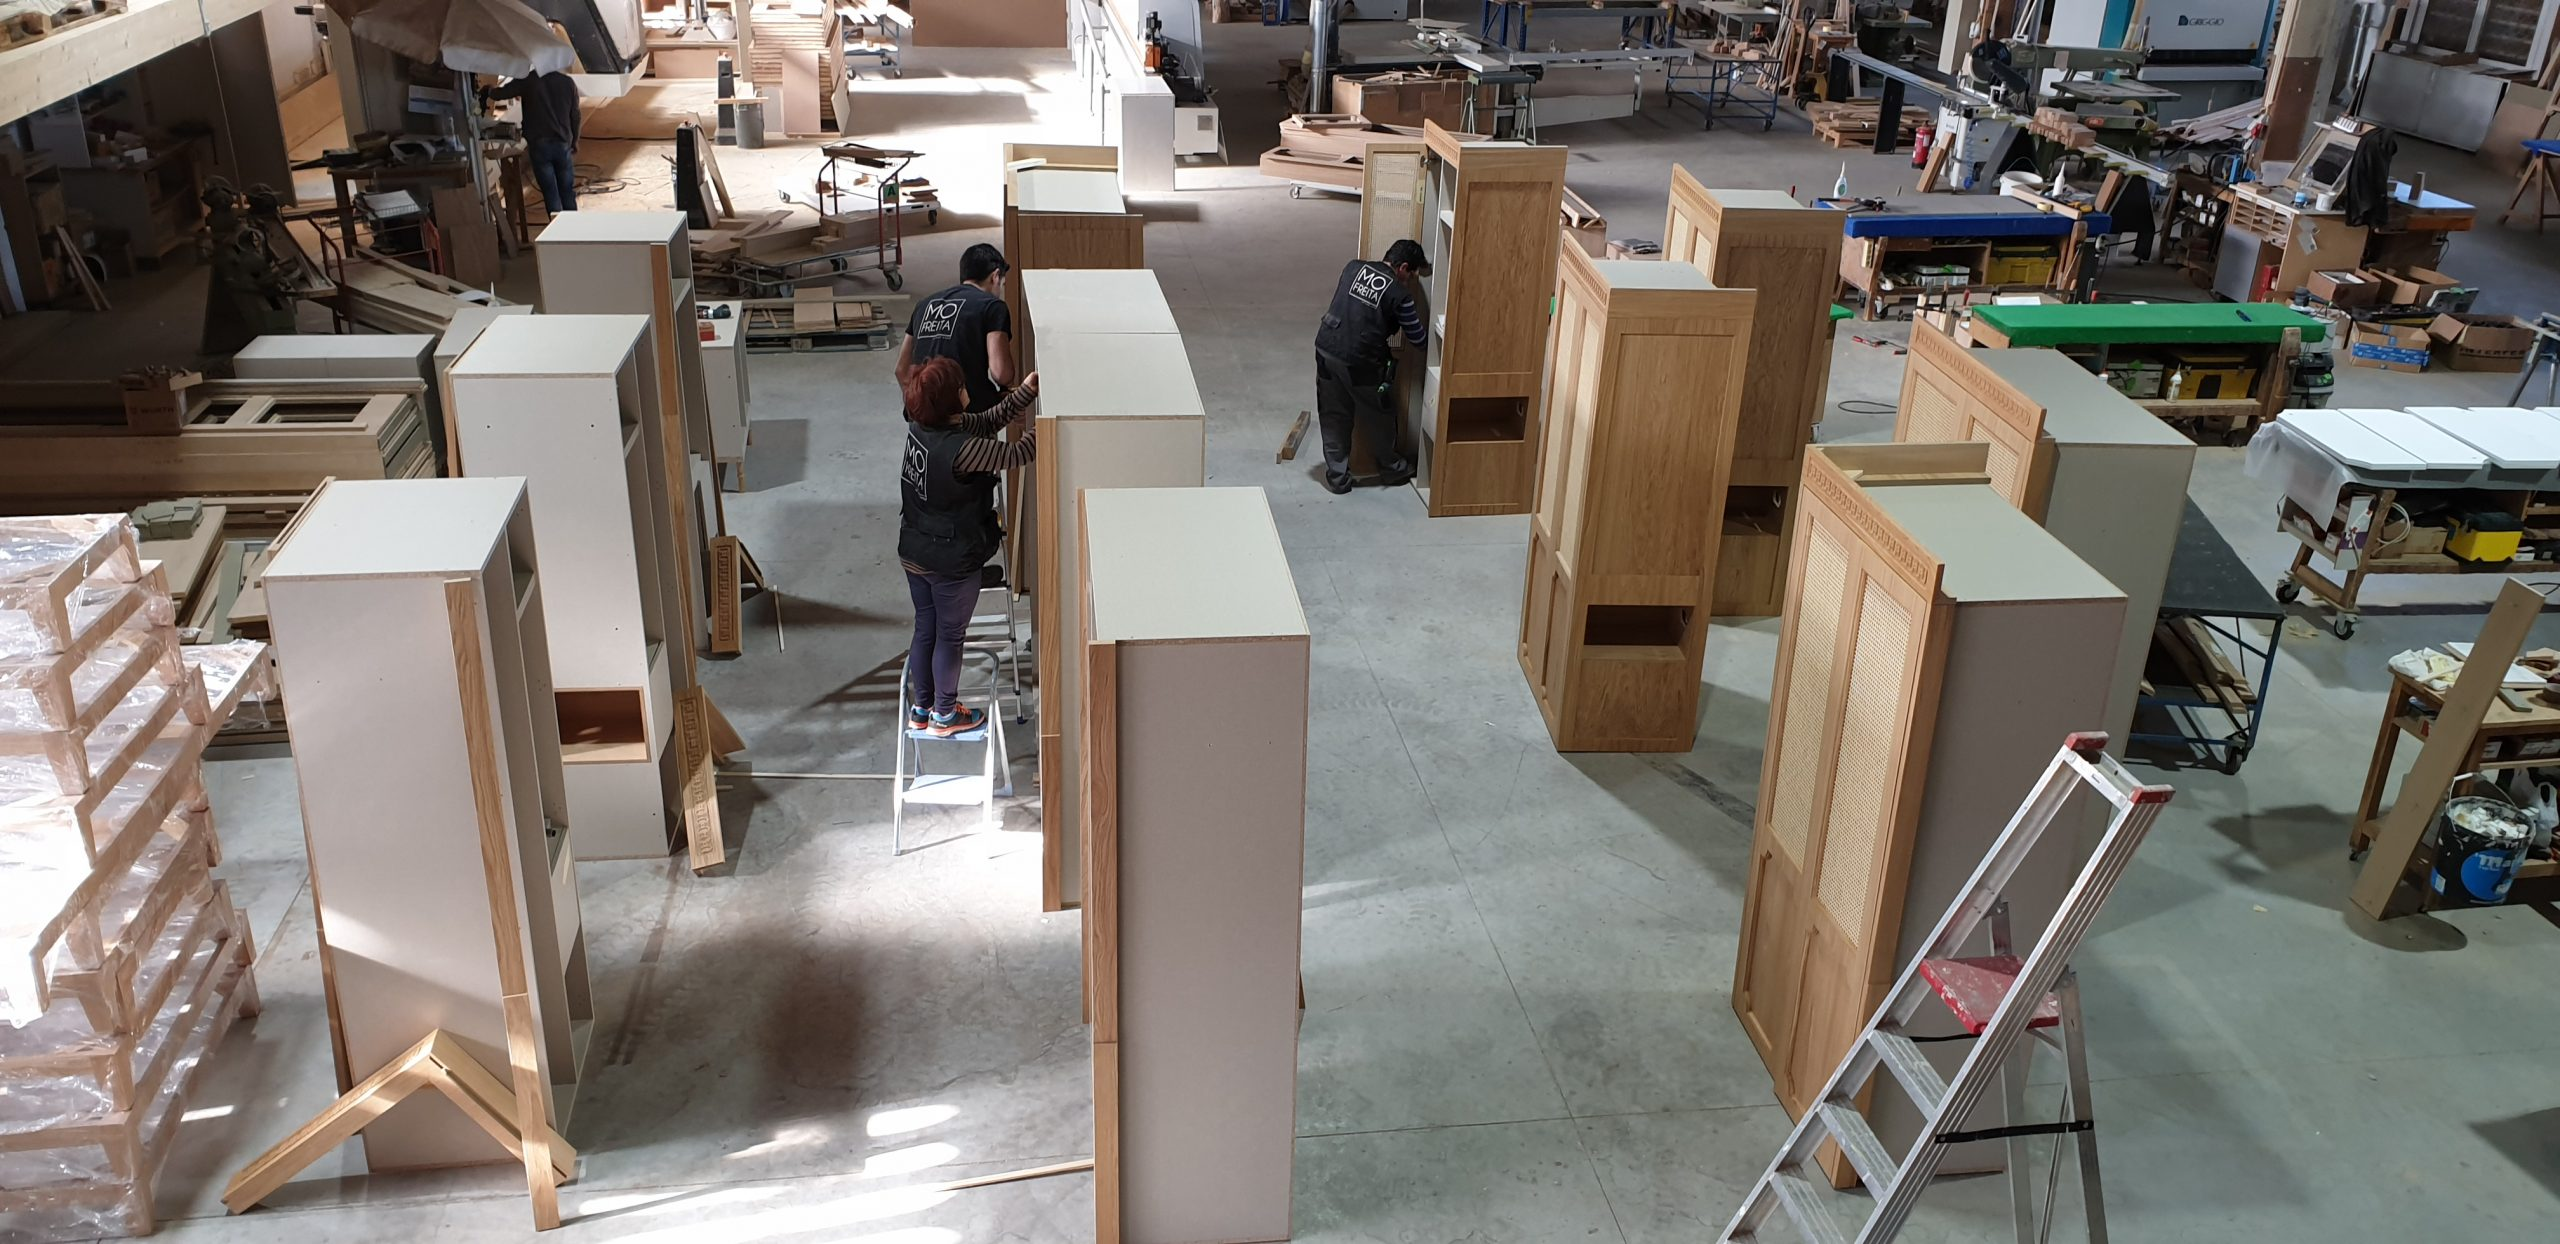
\includegraphics[width=.65\linewidth]{images/Development/chap4/mofreitas.png}
    \caption{Assembly line for wooden furniture at Morefreitas. Source: \cite{noauthor_mofreita_2020}.}
    \label{fig:shopFloor}
\end{figure}




\section{Hardware Architecture}\label{section:hardwareArchitecture}

The electronic architecture overview of the system is based on three modules responsible for keeping the system operating. As shown in Figure~\ref{fig:basicElectronicArchitecture}, the modules are divided in: ultrasonic sensor, microcontroller and power supply. The interaction with the database is not demonstrated in this diagram, as it will be approached, with a deeper discussion, in the Section~\ref{section:database}.

\begin{figure}[h!]
    \centering
    \includegraphics[scale=0.85]{images/Development/hardware_architecture/BasicElectronicSystemArchitecture.pdf}
    \caption{Basic electronic architecture overview.}
    \label{fig:basicElectronicArchitecture}
\end{figure}

The power supply unit consists on a battery, battery charger module and a \gls{DC}-(\gls{DC}) boost converter, responsible for stepping up the voltage.


\subsubsection{Microcontroller ESP32}

Starting with the microcontroller module, the ESP32 Development Board version 1 (see Figure~\ref{fig:esp32}) was selected. Although an Arduino module or, even a Raspberry Pi could be used, the ESP32 was considered due to its size, price and its Wi-Fi onboard feature. The ESP32 is a System-on-Chip (SoC) created by Espressif Systems with integrated Wi-Fi and Bluetooth (BLE) \cite{KURNIAWAN:2019}.

\begin{figure}[h!]
    \centering
    \includegraphics[scale=0.55]{images/Development/hardware_architecture/esp32.pdf}
    \label{fig:esp32}
    \caption{ESP32 Development Kit V1 Board. Image from \cite{datasheet:ESP32}.}
\end{figure}

The ESP32 has a dual core processors and a large numbers of peripherals, e.g., Digital to Analog Converter, Ultra Low Power (ULP) Co-processor, \gls{PWM}, etc. The Wi-Fi and \gls{BLE} operate at 2.4 GHz frequency and it has 34 \gls{GPIO} pins which can be assigned various functions by programming the appropriate registers \cite{datasheet:ESP32}. 

As the ESP32 has a operating voltage which varies from 2.3~V to 3.6~V, the recommended voltage when using a single-power supply is 3.3~V, with an current output of 500~mA or more \cite{datasheet:ESP32}. When the power supply~V\textsubscript{in} receives a \gls{DC} voltage of 5~V, it will automatically turn on the red \gls{LED} D1 and, through the low dropout positive voltage regulator named NCP1117, it will provide to ESP32 an output of 3.3~V \cite{datasheet:NCP1117}. 

Moreover, there is the Micro Universal Serial Bus (USB) which can be used as a power supply and as a USB to Universal Acrychronous Receiver/Transmitter (UART) communication converter integrated. Besides that, the ESP32 development board includes an antenna and antenna matching circuit \cite{datasheet:ESP32}.

Owning so many functionalities and having the Wi-Fi module integrated, the ESP32 is all-rounded chip for the development of \gls{IoT} projects. The development environment setting for ESP32 is provided by Espressif through the \gls{SDK}, which is a bundle of utilities and device-level \gls{API} that enable computer programs to directly communicate with each other, interacting and sharing data \cite{FELKE-MORRIS:2019}. There are several development platforms \cite{ESPRESSIF:ESP32}, e.g., Arduino \gls{IDE}, PlatformIO, Make, ESP-IDF (Espressif \gls{IoT} Development Framework). As demonstrated by \cite{KURNIAWAN:2019}, the ESP32 boards support Arduino development, one of the biggest community for open source hardware and it is chosen to be used for the work development, with the programs of the ESP32 DevKit V1 being written in C language.


\subsubsection{Ultrasonic Sensor US-015}

The US-015 High Accuracy Ultrasonic Sensor, produced by Synacorp Technologies was selected as the ultrasonic sensor module for this work (see Figure~\ref{fig:us015}).

\begin{figure}[h!]
    \centering
    \includegraphics[scale=0.55]{images/Development/hardware_architecture/us015.pdf}
    \caption{US-015 High Accuracy Ultrasonic Sensor.}
    \label{fig:us015}
\end{figure}

The sensor can provide non-contact measurements in a range between 2~cm to 4~m with an operating temperature from 0~ºC up to 70~ºC. The power supply voltage is \gls{DC} 5~V with working current of 2.2~mA, and it has support to \gls{GPIO} communication mode \cite{datasheet:US015}. As presented in Figure~\ref{fig:radiation} (Section~\ref{subsection:influenceOfTheAngle}), an important feature is to have a short detection angle in order to avoid interference from the barrel walls and, the US-015 sensor provides a relative short detection angle within less than 15º. The pin assignments from the US-015 can be seen at the Table~\ref{tab:us015_pin}. 

\begin{table}[h!]
    \centering
    \begin{tabular}{@{}lcc@{}}
        \toprule
         & \textbf{Pin Symbol} & \textbf{Pin Function Description} \\ \midrule
        \rowcolor[HTML]{EFEFEF} 
        1 & Vcc & 5~V Power Supply \\
        2 & Trig & Trigger Input Pin \\
        \rowcolor[HTML]{EFEFEF} 
        3 & Echo & Receiver Output Pin \\
        4 & GND & Power Ground \\ \bottomrule
    \end{tabular}
    \caption{Pin assignments of US-015.}
    \label{tab:us015_pin}
\end{table}

When the ESP32 sends a pulse to the US-015 "Trigger Input Pin" with duration of 30 \begin{math}\mu s\end{math}, the transmitter generates a series of sound waves, the Echo Pin is set to "1" and the time is started to count. After the reflection from the object and the returning to the receiver, the Receiver Output Pin is set to "0". The result is a pulse duration which is equal to the time propagation of the ultrasound wave (see Figure~\ref{fig:us015TimingDiagram}), allowing the distance to be measured.

\begin{figure}[h!]
    \centering
    \includegraphics[scale=0.6]{images/Development/hardware_architecture/us015TimingDiagram.pdf}
    \caption{Ultrasonic timing diagram. Adapted from \cite{ZHMUD:2018}.}
    \label{fig:us015TimingDiagram}
\end{figure}


\subsubsection{Power Supply Module}

The power supply module is composed by the battery, the battery charger and the \gls{DC}-\gls{DC} boost converter. The battery used for this work is the LIR18650 model, with a nominal energy capacity of 2600 mAh, produced by EEMB. Figure~\ref{fig:lir18650} shows the cylindrical lithium-ion rechargeable cell. As described by \cite{datasheet:18650}, the working voltage during the whole discharge process is 3.7~V with an internal impedance of \begin{math}\leq{70}~m\Omega\end{math}.

\begin{figure}[h!]
    \centering
    \includegraphics[scale=0.2]{images/Development/hardware_architecture/lir18650.pdf}
    \caption{Lithium-ion battery model LIR18650 with 2600~mAh.}
    \label{fig:lir18650}
\end{figure}

The Table~\ref{tab:lir18650characteristics} exemplify some basic electrical characteristics of the battery cell when charging and discharging in an ambient temperature of \begin{math}25\pm{5} \end{math}~ºC and relative humidity of \begin{math}65\pm{20}\end{math}~\%.

\begin{table}[h!]
    \centering
    \begin{tabular}{@{}ll@{}}
        \toprule
        Standard Charge & \begin{tabular}[c]{@{}l@{}}Constant Current and Constant Voltage (CC/CV)\\ Current = 520~mA\\ Final charge voltage = 4.2~V\\ Final charge current = 52~mA\end{tabular} \\ \midrule
        Standard Discharge & \begin{tabular}[c]{@{}l@{}}Constant Current (CV)\\ Current = 520~mA\\ Cut-off voltage = 3.0~V\end{tabular} \\ \bottomrule
    \end{tabular}
    \caption{Basic electrical characteristics of LIR18650 when charging and discharging. Taken from \cite{datasheet:18650}.}
    \label{tab:lir18650characteristics}
\end{table}

Since a lithium-ion battery cell is used, a \gls{BMS} needs to be taken in order to enhance safety characteristics \cite{MALGORZATA:2014}. There are several cautions and warnings appointed by the manufacturer in order to provide necessary protection required by lithium batteries \cite{datasheet:18650}. The \gls{BMS} used is the 03962A module (see Figure~\ref{fig:tp4056}), it is made for charging lithium batteries using constant current and constant voltage (CC/CV), moreover, the module provides necessary protection for the batteries, e.g., overdischarge/overcharge protection, overcurrent and short-circuit protection, soft start protection to limit inrush current and trickle charge for battery reconditioning. 

\begin{figure}[h!]
    \centering
    \includegraphics[scale=0.55]{images/Development/hardware_architecture/tp4056a.pdf}
    \caption{TP4056 - 03962A lithium battery charger and protection module.}
    \label{fig:tp4056}
\end{figure}

The battery can be powered, for charging, from the micro USB cable or from the + and - input with \gls{DC} 5~V. Also, the power source needs to be able to provide at least 1~A for correctly charging the connected battery. 

The integrated circuit responsible for the constant-current/constant-voltage linear charger is the TP4056 integrated circuit and it includes several features such as current monitor, under voltage lockout, automatic recharge and two status pin, to indicate charge termination and presence of an input voltage \cite{datasheet:TP4056}. The DW01A and the FS8205A work together in order to protect the battery from damage or degrading the lifetime due to overcharge, overdischarge, and/or overcurrent \cite{datasheet:DW01A, datasheet:FS8205A}.

With the charger module being set, as the nominal voltage during the whole discharge process is 3.7~V and, the final charge voltage is 4.2~V, the battery does not have enough voltage to supply the ESP32 development board and neither the US-015 ultrasonic sensor, while in discharging process, as they both requires a \gls{DC} voltage of 5~V. Because of that, the power supply module requires a \gls{DC}-\gls{DC} boost converter, connected to its output, in order to give a properly power supply for the ESP32 and the US-015. Moreover, the step up converter has a voltage indication, that means the \gls{LED} will be turned on with a load presence and, when the input voltage is lower than 2.7~V, the \gls{LED} indicator will be turned off. 

\begin{comment}
As shown in Figure~\ref{fig:boostPowerSupply}, it is a \gls{DC}-\gls{DC} boost power supply which is responsible for regulating the input voltage to 5~V.

\begin{figure}[h!]
    \centering
    \includegraphics[scale=0.135]{images/Development/hardware_architecture/boost_converter.pdf}
    \caption{DC-DC boost power supply module converter.}
    \label{fig:boostPowerSupply}
\end{figure}


Moreover, the non-isolated step up has a voltage indication, that means the \gls{LED} will be turned on with a load presence and, when the input voltage is lower than 2.7~V, the \gls{LED} indicator will be turned off. 
\end{comment}


\subsection{Electronic Circuit Diagram}

Once presented the necessary electronic components for the hardware architecture development, it is time to show how these components are going to be connected. The Figure~\ref{fig:schematic_projet} illustrates the electronic circuit diagram developed. 

\begin{figure}[h!]
    \centering
    \includegraphics[scale=0.75]{images/Development/hardware_architecture/schematic_project.pdf}
    \caption{Electronic circuit schematic of the project.}
    \label{fig:schematic_projet}
\end{figure}

As the ESP32 is going to receive a signal from the Echo Pin that may be "1" or "0", as described in Figure~\ref{fig:us015TimingDiagram}, they do not need an analogic-to-digital converter. Therefore, the ultrasonic sensor pins can be directly connected to any \gls{GPIO} of the ESP32 development board. Thereby, the trigger pin of the ultrasonic sensor is connected to the \gls{GPIO} D15 of the ESP32 board and, the echo pin is connected to the \gls{GPIO} D4. Also, the \gls{DC}-\gls{DC} boost converter is power supplying to both ESP32 board and the US-015 ultrasonic sensor.


\section{Enclosure Design}

As demonstrated in Figure~\ref{fig:deviceModelPosition}, the solution adopted is to create a custom-made hardware enclosure
that allows the measurements to be taken from a top position of the barrel. Therefore, the enclosure must be able to thread, into one of the openings, and it must allow that all the electronic components can be fitted in a well organized and structured manner, allowing the wiring connections to be made as clean as possible. The enclosure was first drawn by using the software SolidWorks version 2017/2018. 

Starting with the screw thread, the measurements used for the software design were taken from the bung cap, as shown in Figure~\ref{fig:plasticDrumCaps}. As it was difficult to find the exactly measures, due the lack of information about the maker of the plastic drum barrels and bung caps, it was necessary to perform the measurements manually using a digital caliper.

\begin{figure}[h!]
    \centering
    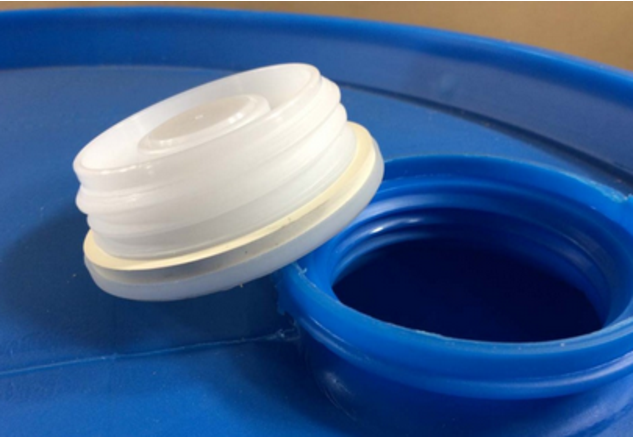
\includegraphics[scale=0.8]{images/Development/3D_device_development/plasticDrumCaps.pdf}
    \caption{Plastic drum screw cap.}
    \label{fig:plasticDrumCaps}
\end{figure}

It is important to have some basic considerations when designing a screw thread. First, as demonstrated in Figure~\ref{fig:screwThreads}, the pitch is given by the distance between the crests, the major diameter is the diameter of the imaginary co-axial cylinder that touches the crests and, for the minor diameter is the imaginary cylinder that touches the grooves. Also, the length of the screw is important in order to know how many revolutions the screw thread will have.

\begin{figure}[h!]
    \centering
    \subfigure[Screw thread measurements overview.]{
        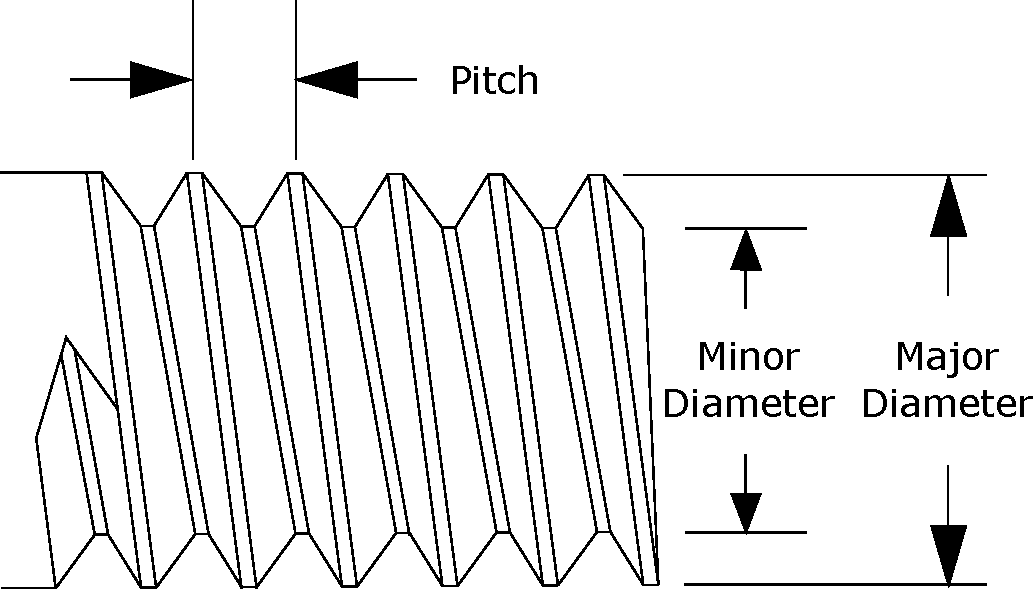
\includegraphics[scale=0.44]{images/Development/3D_device_development/screwThread.pdf}
        \label{fig:screwThreads}
    }\quad\quad
    \subfigure[Basic profile of the screw threads.]{
        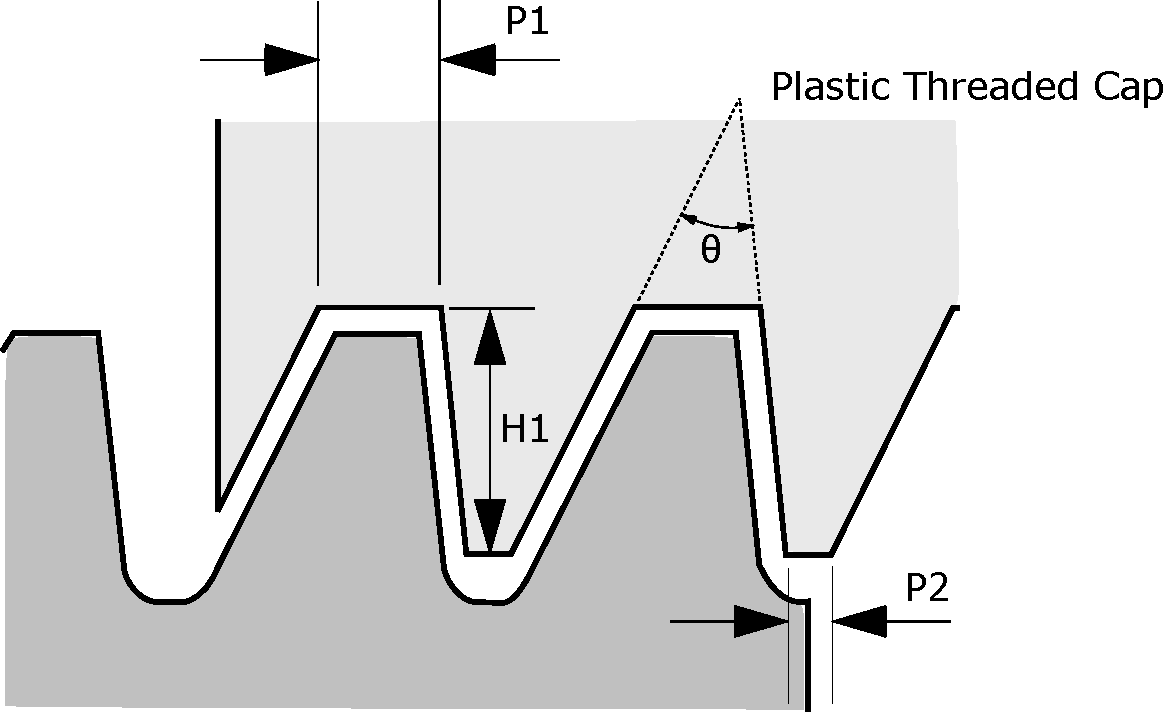
\includegraphics[scale=0.35]{images/Development/3D_device_development/busttressScrewThreads.pdf}
        \label{fig:buttressScrewThreads}
    }
    \caption{Basic plastic screw threads considerations.}
    \label{fig:threads}
\end{figure}

Already for the Figure~\ref{fig:buttressScrewThreads}, it is showing a basic profile of a screw thread. The measures P1 and P2, the height H1 and the angle \begin{math}\theta\end{math} of the screw thread are important measurements in order to have a good fit between the parts.

Ensuring these considerations, a design of screw cap can be made. As shown in Figure~\ref{fig:buttressDesign}, it is demonstrating the front and isometric view of the screw thread.

\begin{figure}[h!]
    \centering
    \subfigure[Front view.]{
        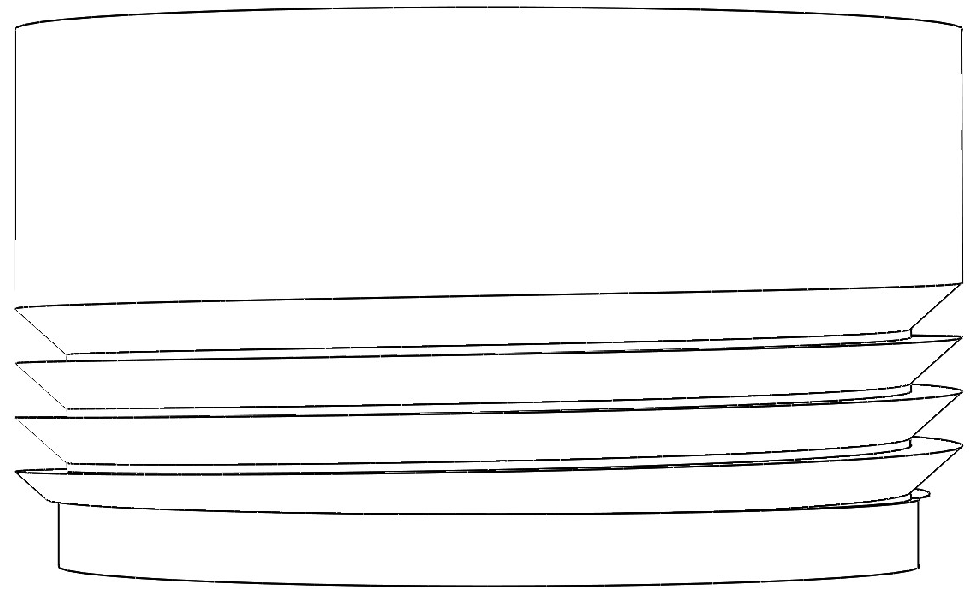
\includegraphics[scale=0.3]{images/Development/3D_device_development/screw1.pdf}
        \label{fig:frontViewButtress}
    }\quad\quad\quad\quad\quad\quad
    \subfigure[Isometric view.]{
        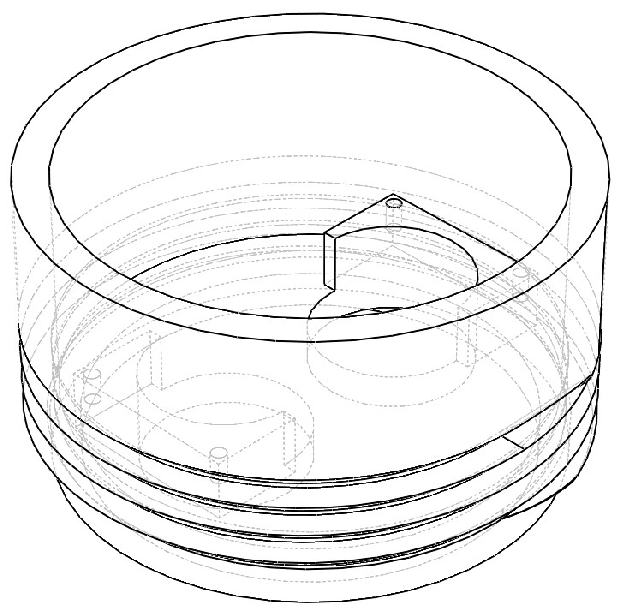
\includegraphics[scale=0.35]{images/Development/3D_device_development/screw2.pdf}
        \label{fig:isometricViewButtress}
    }
    \caption{Overview of the screw thread design.}
    \label{fig:buttressDesign}
\end{figure}

As can be noticed from Figure~\ref{fig:isometricViewButtress}, inside of the screw there must be two openings that allows the ultrasonic sensor to take readings from the liquid surface. Then, using the Fusion3 F400 3D printer, the screw thread designed is printed and the 3D model is proceeded to be tested on the plastic drum barrel (see Figure~\ref{fig:3DscrewThead}).

\begin{figure}[h!]
    \centering
    \includegraphics[scale=0.14]{images/Development/3D_device_development/screwThreadTest.pdf}
    \caption{Printed 3D screw thread being tested.}
    \label{fig:3DscrewThead}
\end{figure}

Thus, the electronic components is drawn in solid model and is used in order to have a better understanding about the dimensions and design of the whole device model. In Figure~\ref{fig:preview3Dmodell}, it is shown a preview model of the whole device. From the front view in Figure~\ref{fig:frontViewPreviewModel}, there are two access openings, one for the micro USB module charger and one for the ESP32. In the middle, it will be placed a switch button for turning the device ON and OFF. The openings from the side view, in Figure~\ref{fig:sideViewPreviewModel}, are for the ESP32 onboard \gls{LED}s, responsible for alerting if the device is powered up and for the alert system, warning in case the liquid's surface is under a predetermined value.

\begin{figure}[h!]
    \centering
    \subfigure[Front view.]{
        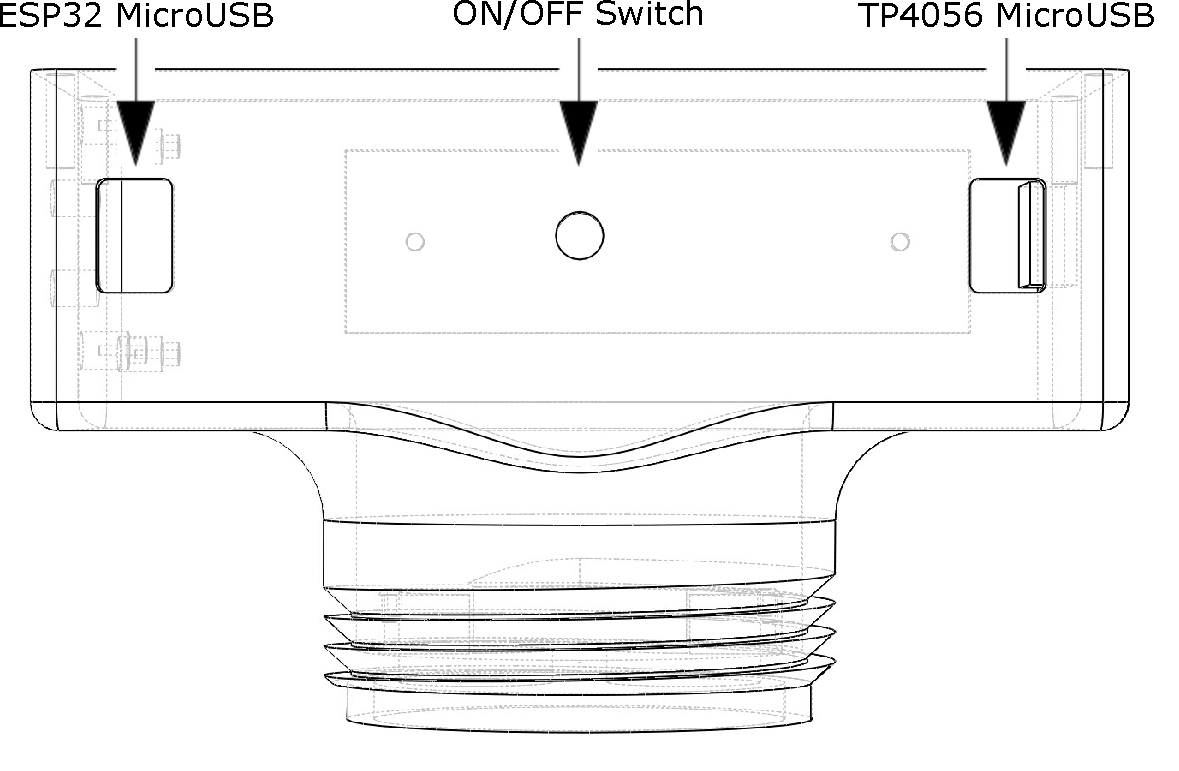
\includegraphics[scale=0.35]{images/Development/3D_device_development/3dFrontView.pdf}
        \label{fig:frontViewPreviewModel}
    }\quad\quad\quad\quad
    \subfigure[Side view.]{
        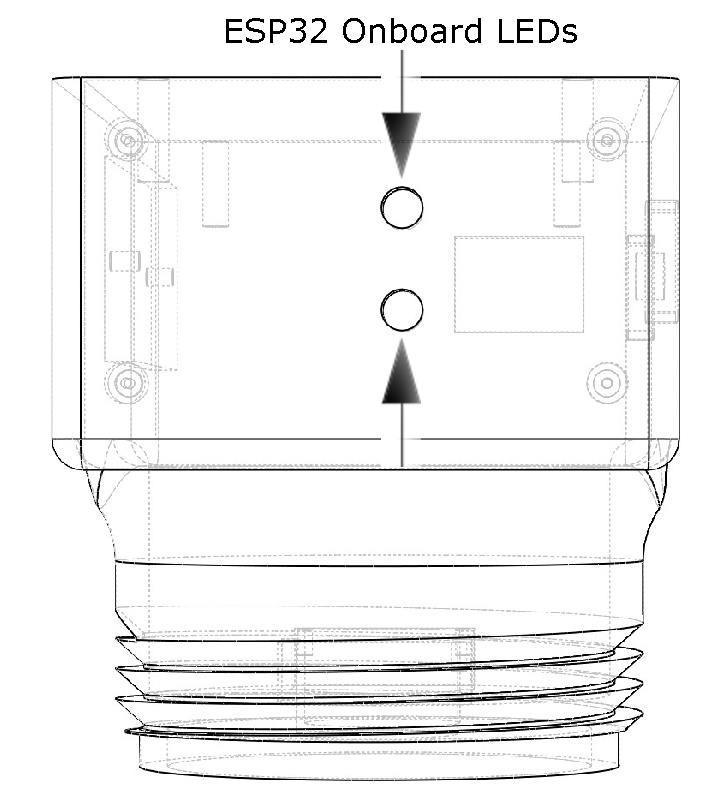
\includegraphics[scale=0.35]{images/Development/3D_device_development/3dSideView.pdf}
        \label{fig:sideViewPreviewModel}
    }
    \caption{Preview of the 3D device model.}
    \label{fig:preview3Dmodell}
\end{figure}

Therefore, the final version of the device is demonstrated in Figure~\ref{fig:3DmodelDevice}. As can be viewed, the device has a cover which is secured by 4 screws located at the corners. Already for the Figure~\ref{fig:positionEletronicComponents}, it is shown the position of the electronic components inside of the model.

\begin{figure}[h!]
    \centering
    \subfigure[Isometric view of the device.]{
        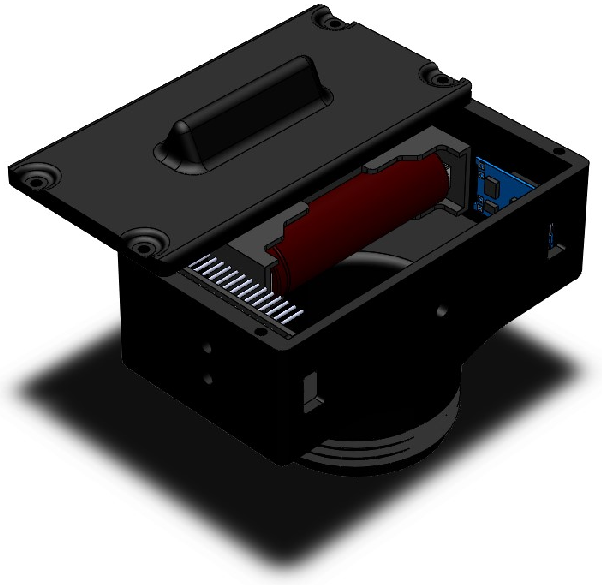
\includegraphics[scale=0.58]{images/Development/3D_device_development/3dFinalVersion.pdf}
        \label{fig:isometricViewDevice}
    }
    \subfigure[Position of the electronic components in the device.]{
        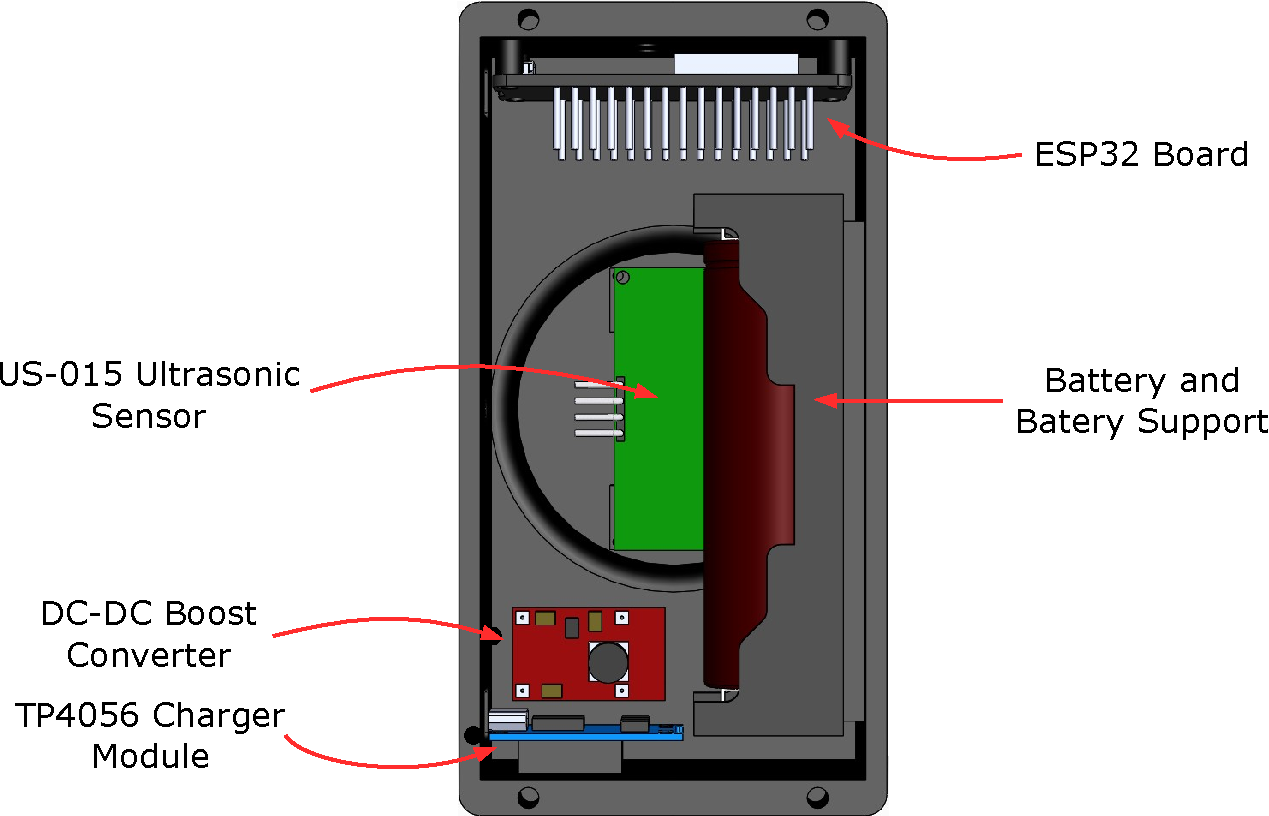
\includegraphics[scale=0.43]{images/Development/3D_device_development/3dFinalVersionTop.pdf}
        \label{fig:positionEletronicComponents}
    }
    \caption{Final device model.}
    \label{fig:3DmodelDevice}
\end{figure}

Now that the device model is defined, it is time for the printing process. The printer uses the Simplify3D software control, which is responsible for translating the 3D models into instructions that the printer can understand. There are a wide range of information on their website in order to have better printing results. Mainly, regarding the support structures. The printed model can be seen in Figure~\ref{fig:3dDPrintedDevice}, in which PLA (short term for Polylactic Acid) filament was used as the material for the printed model.

\begin{figure}[h!]
    \centering
    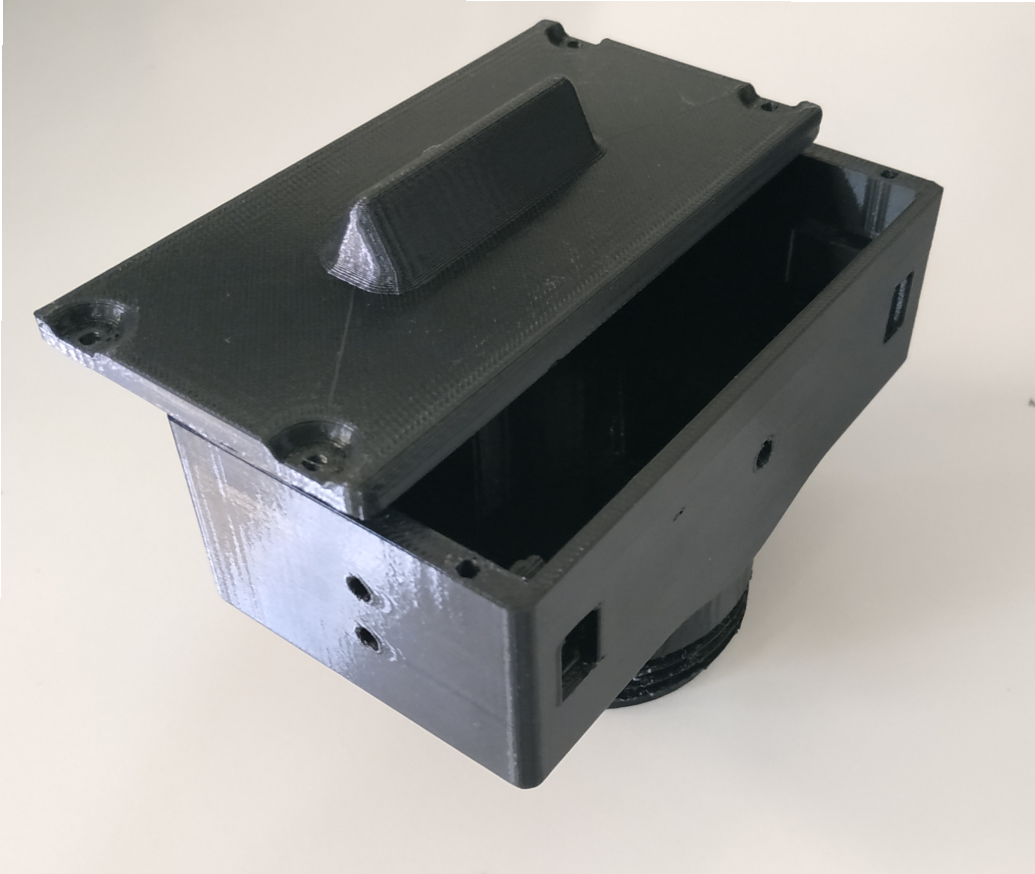
\includegraphics[scale=0.43]{images/Development/3D_device_development/PrintedModel.pdf}
    \caption{3D printed model.}
    \label{fig:3dDPrintedDevice}
\end{figure}

After all the printing process, it is time to install the electronic components inside the printed device. Following the electronic circuit schematic, as illustrated in Figure~\ref{fig:schematic_projet}, the implementation resulted is shown in Figure~\ref{fig:final3Dmodel}.

\begin{figure}[h!]
    \centering
    \subfigure{
        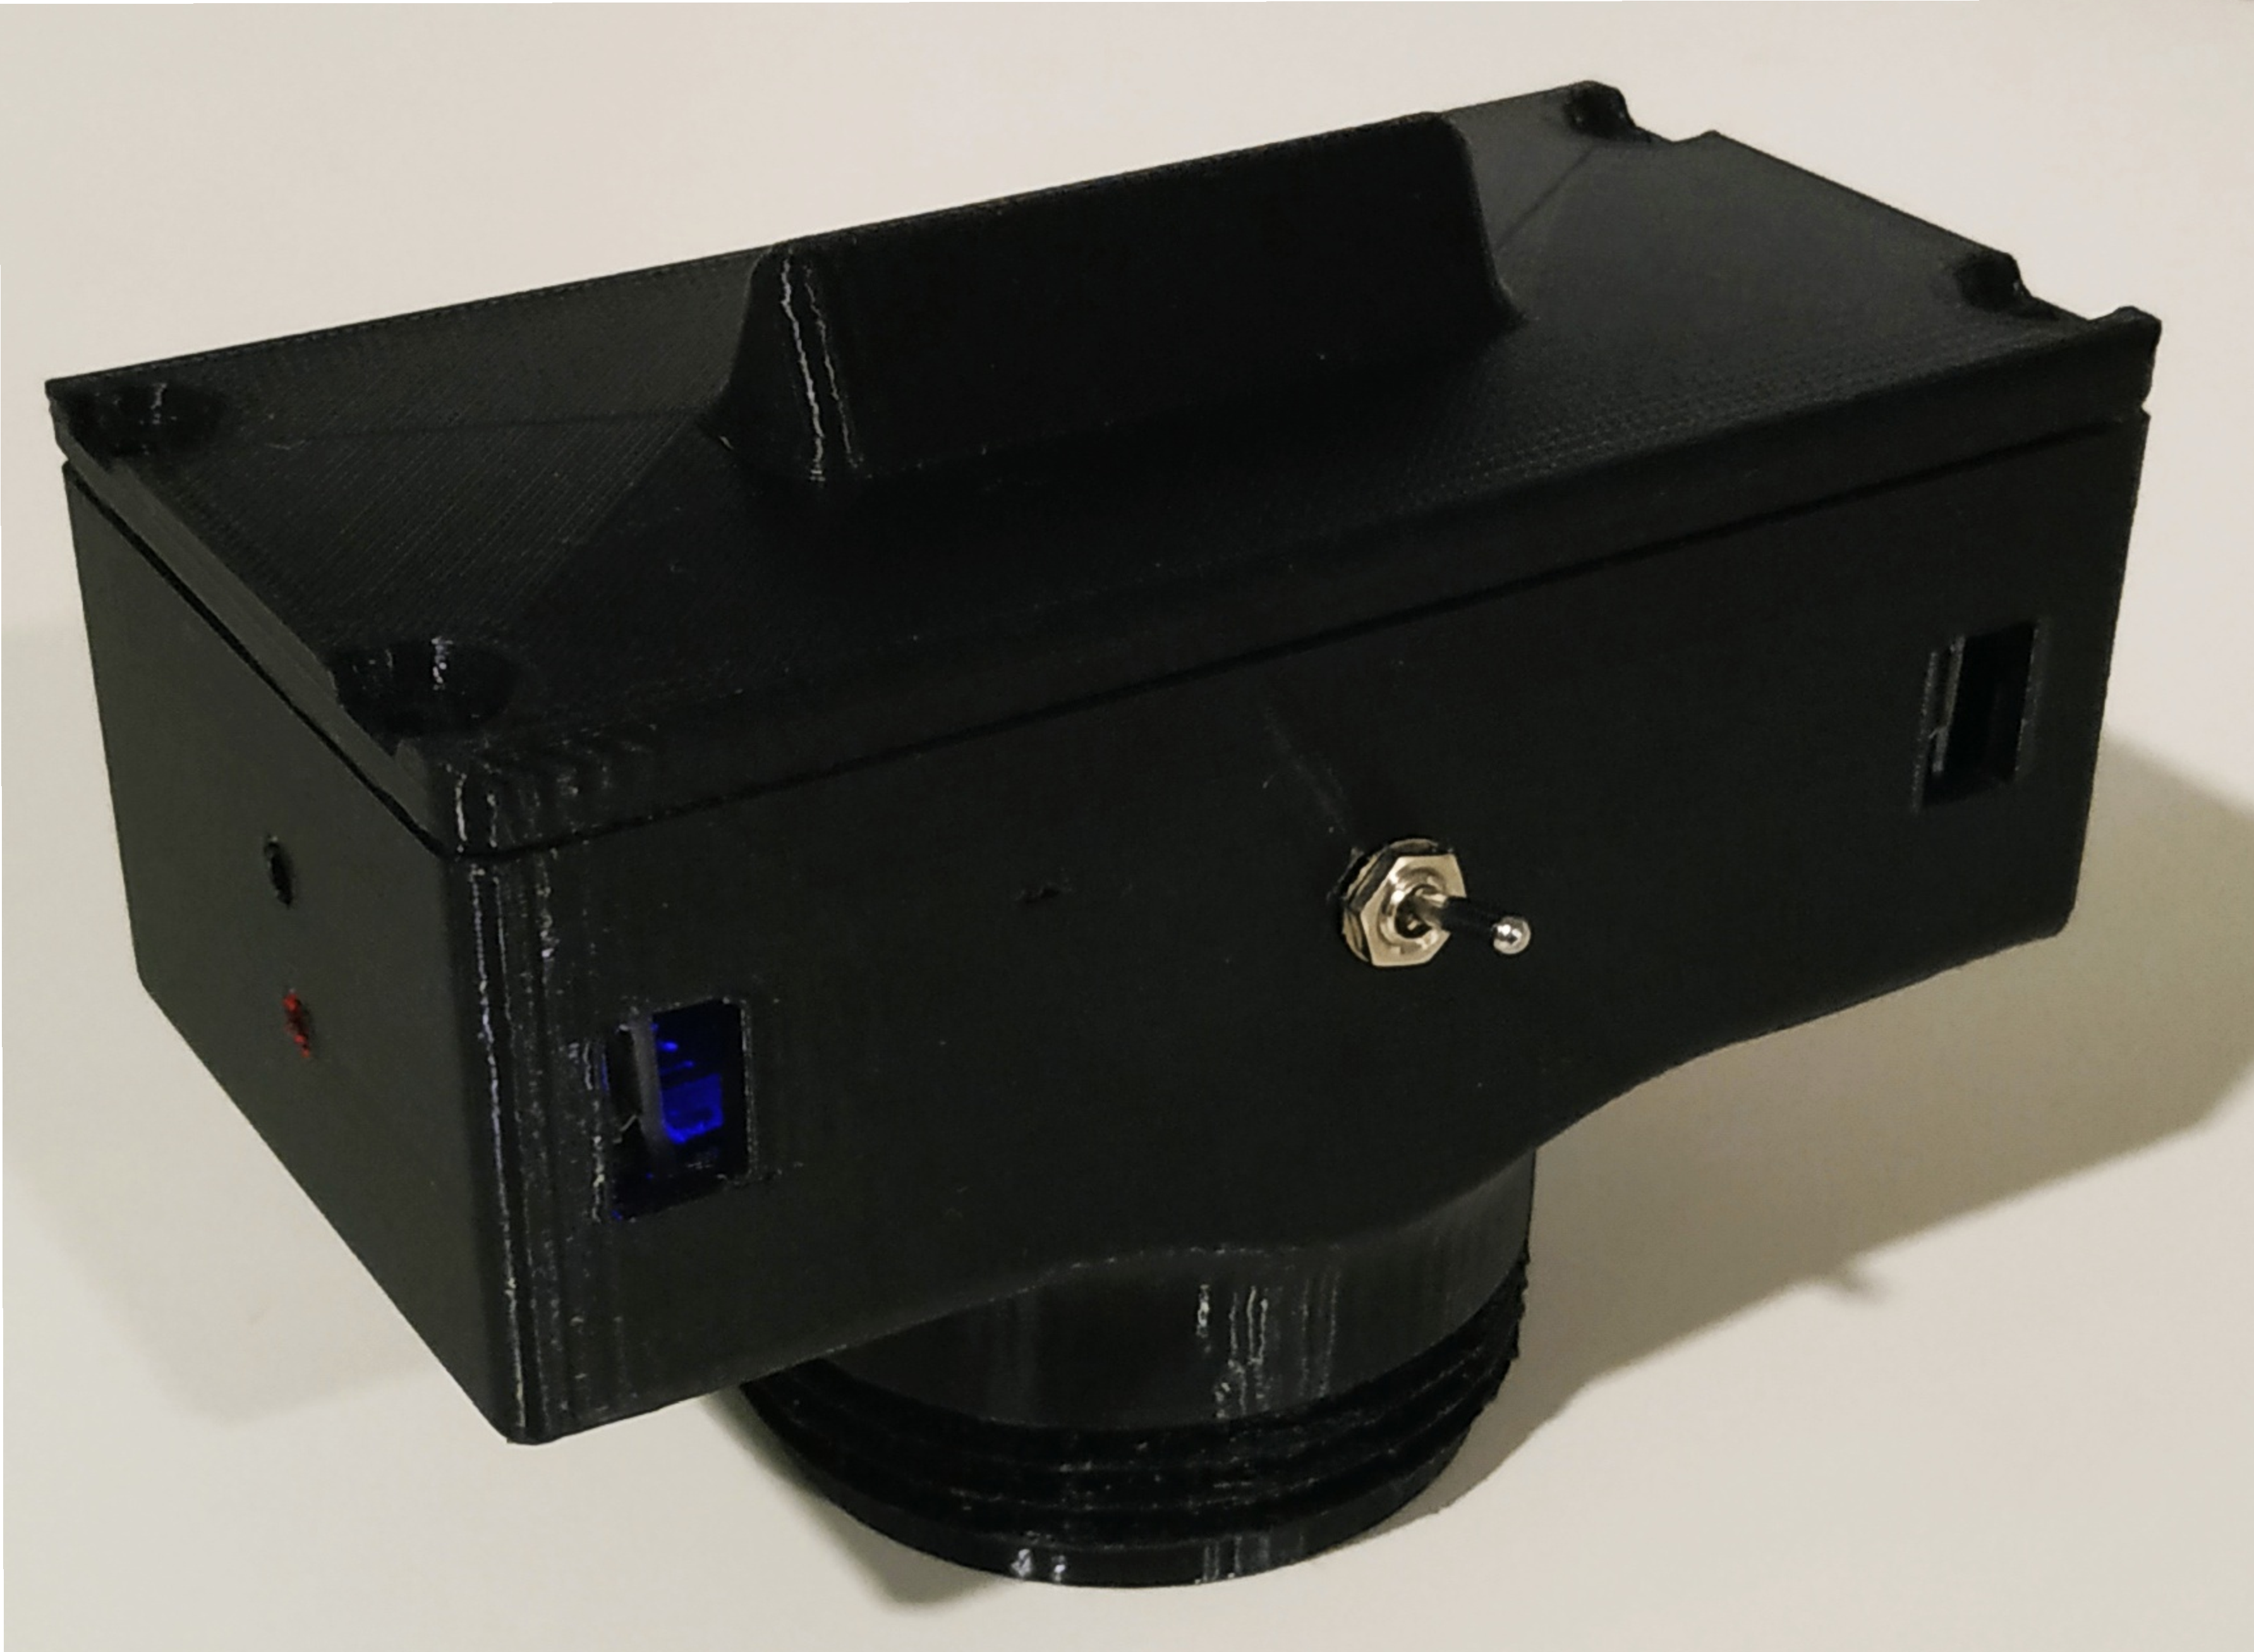
\includegraphics[scale=0.117]{images/Development/3D_device_development/3DPrintedModelFinal.pdf}
        \label{fig:uncovered}
    }
    \subfigure{
        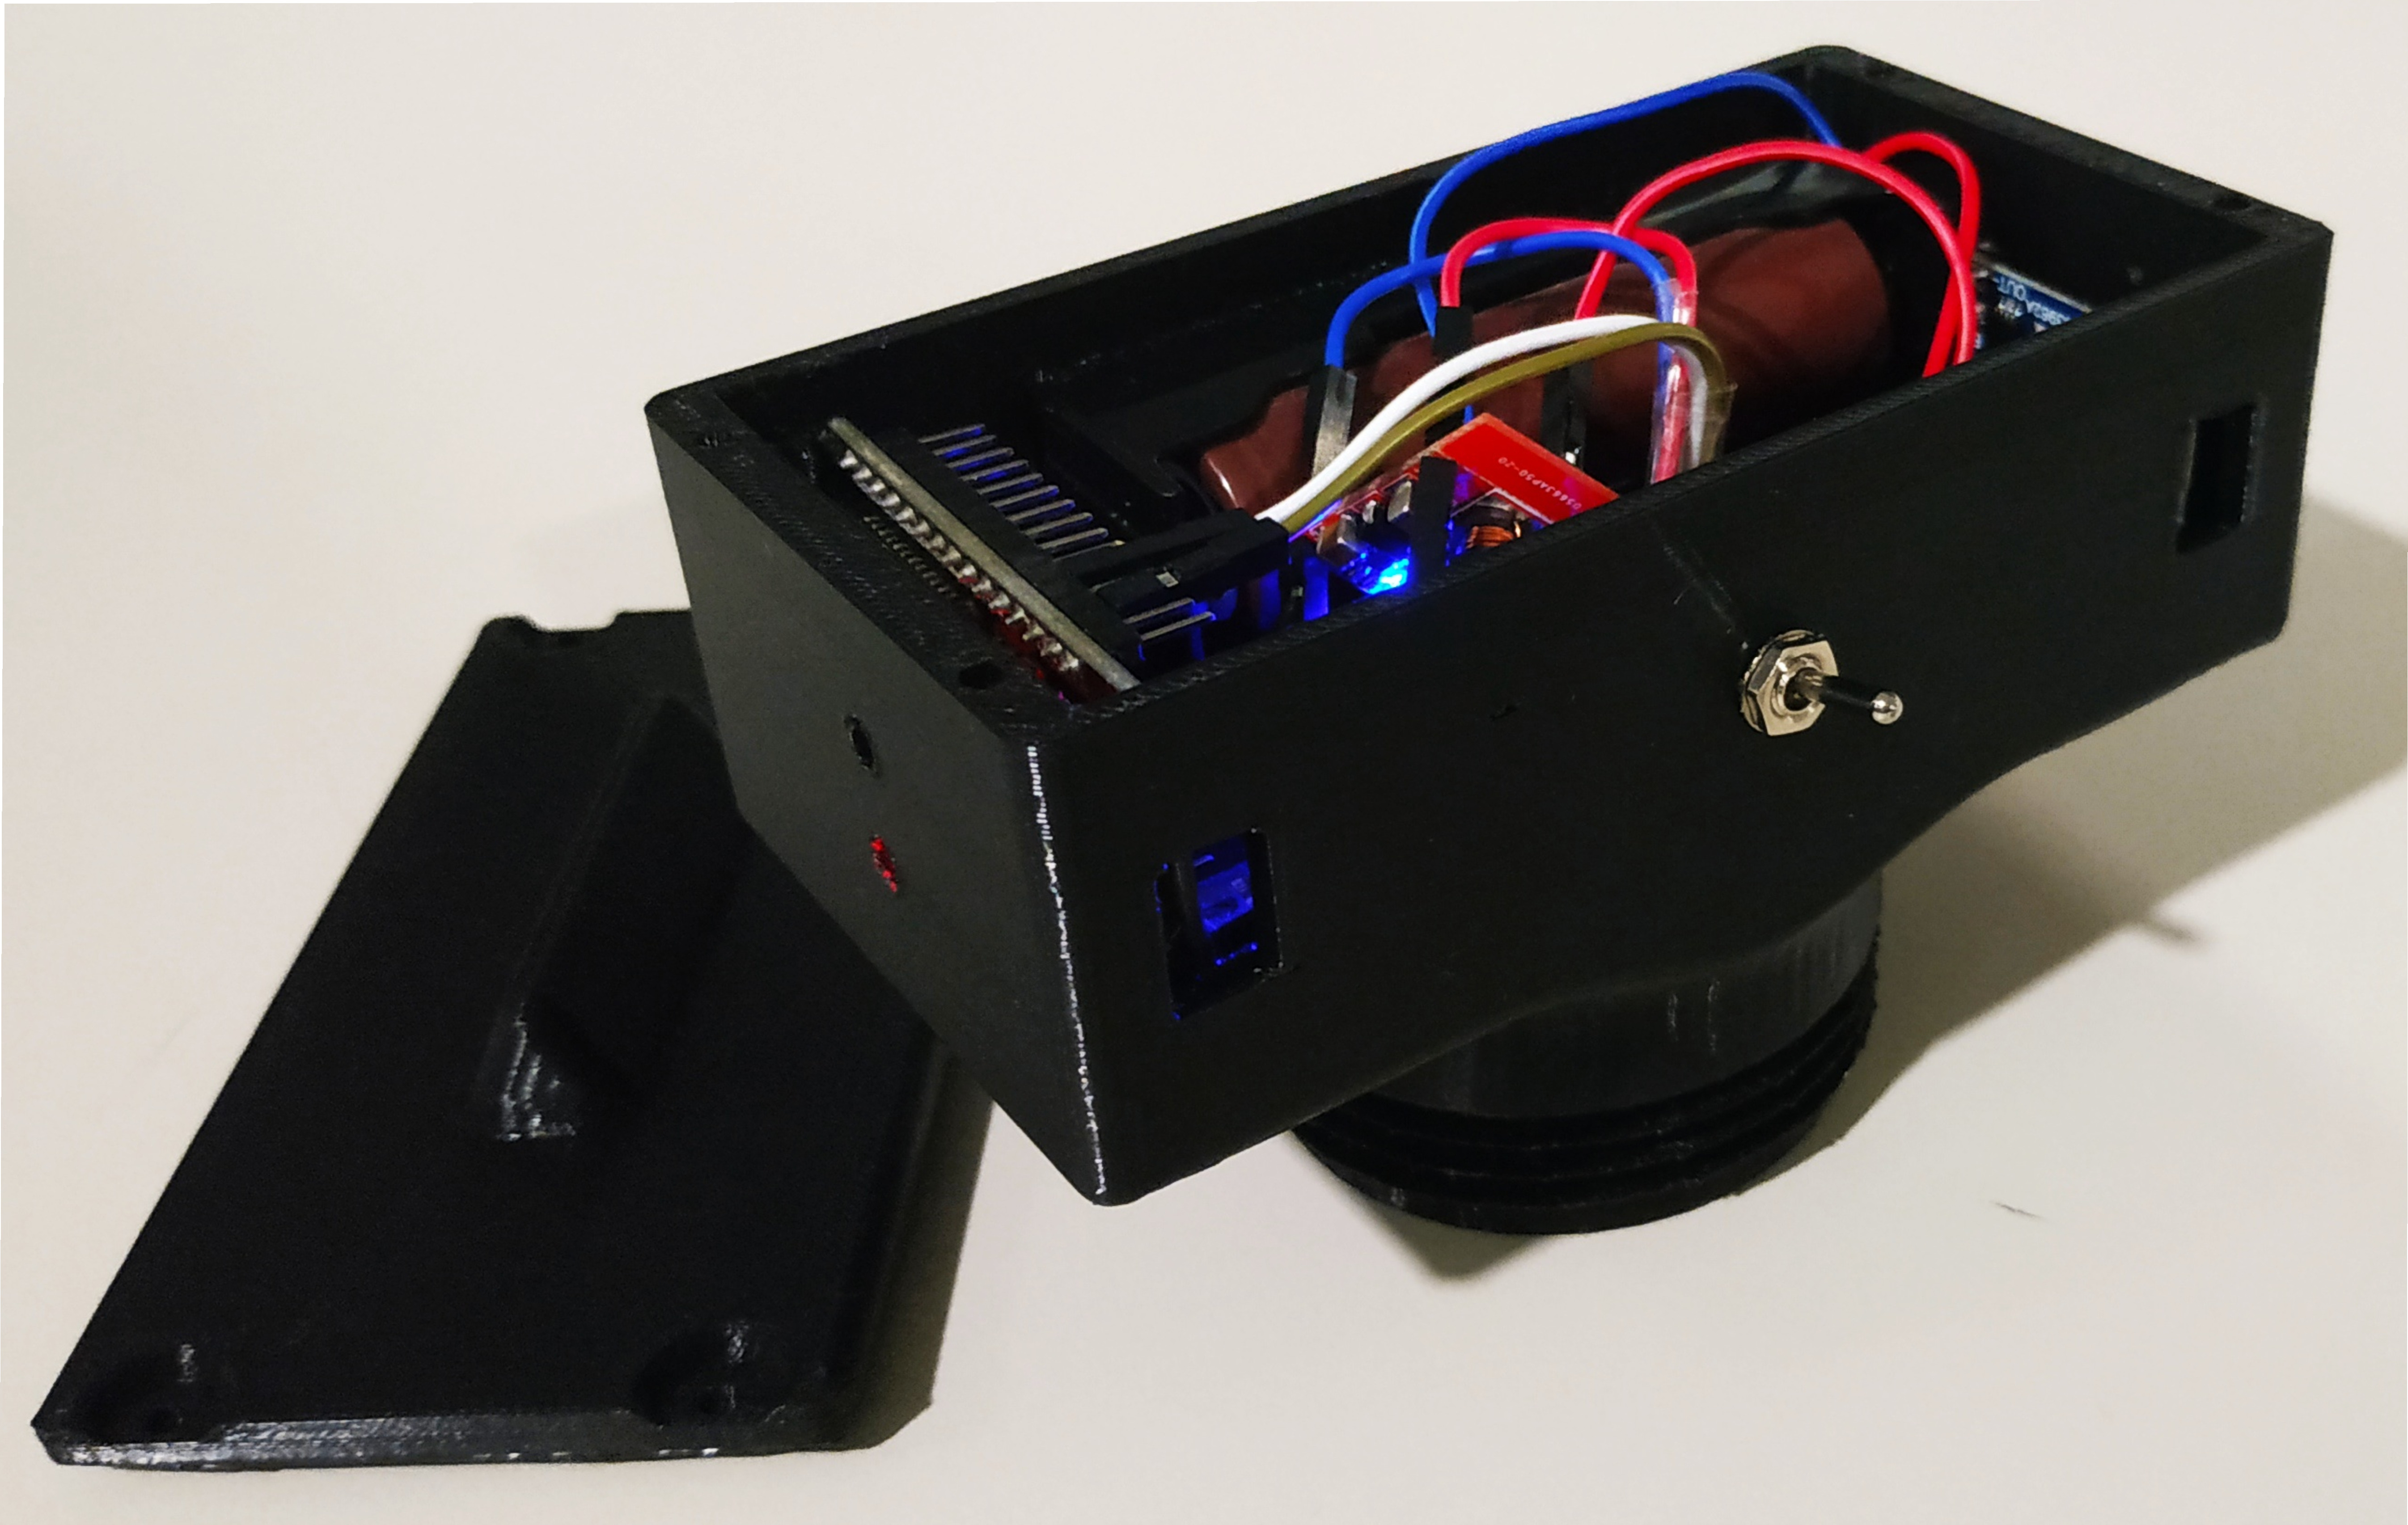
\includegraphics[scale=0.09]{images/Development/3D_device_development/3DPrintedModelFinalUncover.pdf}
        \label{fig:covered}
    }
    \caption{Final version of the 3D printed device.}
    \label{fig:final3Dmodel}
\end{figure}


\section{Setting up the ESP32}\label{section:settingESP32}

In this section, it is demonstrated the software development responsible to retrieve and manage the ultrasonic measurements. The development environment used to program the ESP32 Board is the Arduino \gls{IDE}, the installation of the board in the software can be done by following the steps provided by \cite{KURNIAWAN:2019} or directly in \cite{ESPRESSIF:ESP32}. After it is established the programming tool, it is time to define the characteristics adopted for the system and the flowchart overview of how the embedded software works. 


\subsection{Software Design}

Starting with the Wi-Fi configuration, it refers to the information related to the name of the Wi-Fi network (SSID), the password and the \gls{IP} host address, responsible for allowing the connection between the client and the server, where the data will be stored. 

Analyzing the barrel characteristics, it is adopted the diameter, height and volume. As there is no mathematical model that describes exactly the geometry of the barrel, it is used the Equation~\ref{eq:totalVolume} for the volume calculation.

The alert system is responsible for emitting a light warning, by turning on an ESP32 onboard \gls{LED}, in which it will inform the managements when the barrel capacity is less then a predetermined value. The \gls{LED} will maintain its state until the capacity of the sensor is above the predetermined value.

Another feature is the check system, which is responsible for saving the old value of the distance measured, in the internal memory of the ESP32, in order to compare with the new value, before the information is sent to the database. This prevention system is important for level measurement systems, specially when the liquid level to be measured does not change quickly between two consecutive measurements. Thereby, it avoids possible nonsense values to be send to the database, by comparing them before the data to be sent.

For the environment temperature, as all reservoirs are located at centralized in a room inside the facilities of the \gls{SCMB} and, each plastic barrel has only two openings, as shown in Figure~\ref{fig:topViewBarrel}, due the material of the plastic barrel and the location where they are placed, it is assumed that the average temperature is closely to constant.

Furthermore, the system has a variable which allows to define a number of samples. This variable is responsible for the US-015 ultrasonic sensor to take successively measurements, in a short period of time, with the objective to decrease the errors from the readings. 


\subsubsection{Measurement System Flowchart}

The flowchart of the sensor readings are shown in Figure~\ref{fig:flowchartUltrasonicReadings}. It is basically responsible for retrieving, avoiding and treating the ultrasonic sensor readings, calculating and returning the distance, volume and capacity of the barrel's liquid.

\begin{figure}[h!]
    \centering
    \includegraphics[scale=0.85]{images/Development/Setting_the_ESP32/flowchart_ultrasonic_readings.pdf}
    \caption{Flowchart of the ultrasonic sensor readings.}
    \label{fig:flowchartUltrasonicReadings}
\end{figure}

This function makes the ESP32 to send a pulse to the trigger pin of the US-015 with a period of 30~\begin{math}\mu s\end{math}, than it will wait for the echo answer with a timeout of 60~ms. At this point, the time is being counted. 

If the echo exists, the system will make another process to check if the returned time value is appropriate or not. In case the time is appropriate, the system will make the distance calculation, using the Equation~\ref{eq:distanceCm}, and the result will be stored in a auxiliary vector. However, if the time value is not appropriate, the ESP32 will send a low pulse to the echo pin of the US-015 in order to reset the readings received from the echo pin, preventing the system to make new readings with the same errors, due to interference factors.

The system will make repetitively measurements until the number of samples is reached. After this point, all the measurements stored in the auxiliary vector will be added and the distance mean will be calculated. Thus, the volume and capacity is calculated with the Equations \ref{eq:liquidVolume} and \ref{eq:capacity}, respectively, and the parameters are returned from the function.


\subsubsection{System Flowchart}

Upon the completion of the software design, Figure~\ref{fig:flowchart_esp32} demonstrates the flowchart of the code written and programmed into the microcontroller, it also can be found by checking in \cite{COELHO:2019}. It begins with the initialization of the parameters presented in the previous section and the libraries necessary for the development of the program.

\begin{figure}[h!]
    \centering
    \includegraphics[scale=0.9]{images/Development/Setting_the_ESP32/flowchart_esp32.pdf}
    \caption{The system flowchart.}
    \label{fig:flowchart_esp32}
\end{figure}

The libraries used are the <Wi-FiClient.h> and the <WebServer.h>, they enable the ESP32 Board to connect with a Wi-Fi network and sending information through \gls{HTTP} request method. Following, the system defines the pin mode and, makes reads from the ultrasonic sensor module, as shown in Figure~\ref{fig:flowchartUltrasonicReadings}. Thus, the distance returned is stored in an auxiliary vector for further comparisons. Lastly, the microcontroller connects to a local Wi-Fi network.

Already inside of the infinite loop, the system will update the distance value stored at the auxiliary vector by making new readings from the sensor, then, it makes an absolute difference between the old and new values. The system will make five comparisons if the distance difference is greater than 10.00 cm. In case after this five comparisons, the system continues providing this big difference, the system will decide that this value is true and it will continue with the program flow. Otherwise, the value will be discarded and the system will be forced to do other readings, from the sensor module, in order to check if the value measured is correct.

After these strict comparisons, the system will make some basic checkup and it will print, through the serial monitor, specific alerts in case of nonsense values. Then, the system will rerun the program until a reasonable distance measurement is taken.

Starting the checkup process with the US-015 ultrasonic sensor, as it is capable of doing measurements in a range of 2~cm to 4~m, the system will print \textit{Invalid measurement!} when the distance is shorter then 2.0 cm and, for the maximum operating range of the sensor, it will be limited to the barrel's height. Thereby, in case the distance measured is greater, the sensor will print a message \textit{Connect the Sensor at the Barrel!}, as it is impossible for the system to detect a higher measurement than it is. Lastly, it is verified if the distance is a number or not, in case this function is true, it will be printed \textit{Failed to Read From the Sensor!}.

At this point, the distance measured is valid and the values of the distance, volume and capacity is ready to be sent for the database. It will blink a LED, alerting that the system took the measurements, and it is about to send the data to the database. Finally, the Alert Function will turn on the ESP32 onboard \gls{LED}, in case the capacity parameter is under a predetermined value, and the values will be printed in the serial monitor. 

Following, the client makes a request by using the GET method, which is one of the \gls{HTTP} methods used to indicate that a desired action is to be performed. The action is to communicate with an \gls{API} responsible for inserting the data in a \gls{RDBMS}. The distance, volume and capacity information are passing in the form of an entity embedded in the \gls{URL} where the database server is located.

Lastly, the ESP32 board will go into a sleep state and it will remain for a while until further measurements are required. The delay time can be set according to the application necessities.


\section{Database Development}\label{section:database}

Upon to complete the review of the whole system development, this last section approach the structure of the database, the \gls{API}s and the developed web pages \cite{COELHO:2019}. As they are hosted on server, it was chosen \textit{000webhost} services, which is a free web hosting fully-functioning with \gls{PHP} and My\gls{SQL} features. The disk space available is up to 1 GB with 10 GB of bandwidth, which is more than enough for development and testing the laundry integrated system.

The Figure~\ref{fig:databaseArchitecture} illustrates the server architecture overview. As can be seen, the \gls{API}s communicate either with the database and the Web pages, allowing the users to access the database content, dynamically and interactively, through the \gls{HTML} Web pages.
 
\begin{figure}[h!]
    \centering
    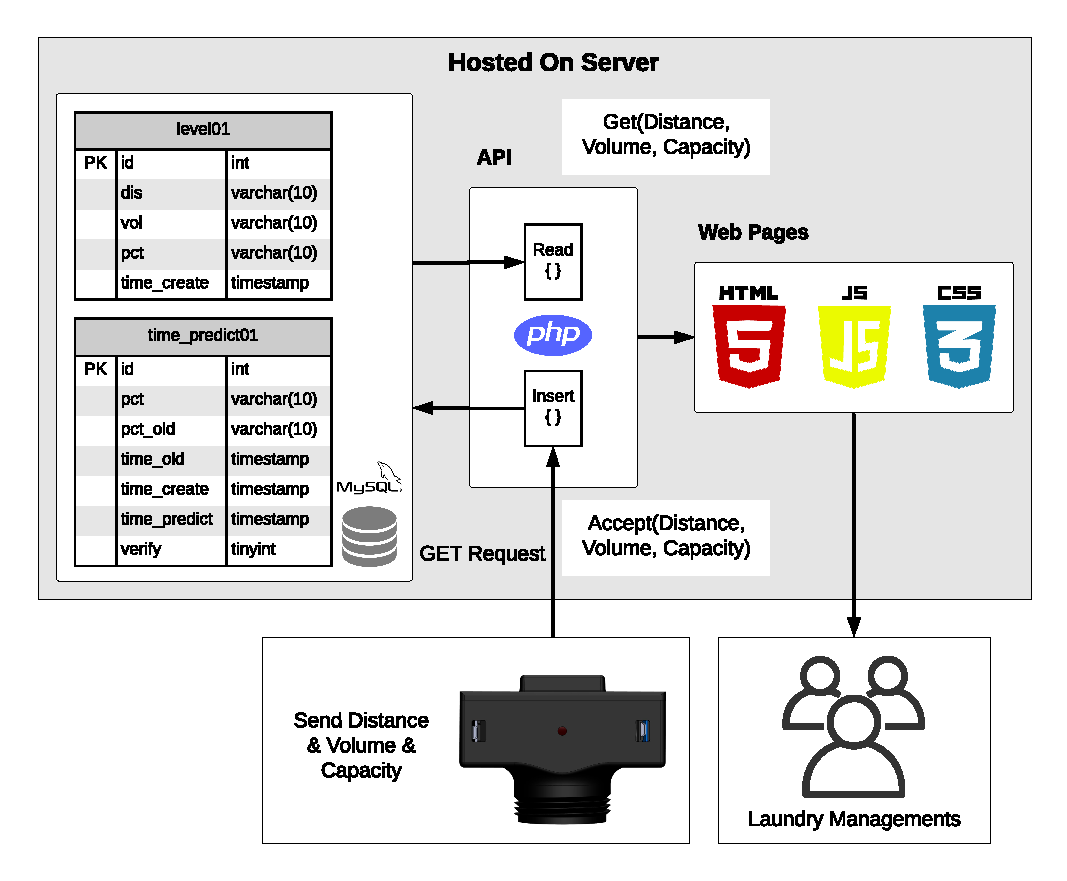
\includegraphics[scale=0.75]{images/Development/web_database/database_overview.pdf}
    \caption{Web database architecture overview.}
    \label{fig:databaArchitecture}
\end{figure}

Although the Figure~\ref{fig:databaseArchitecture} is showing only two \gls{API}s, one for inserting data in the tables and another for making readings, in practice, the structure is a little bit more complex. In order to understand how the database structure works, it is necessary to make an overview about the website flowchart and the \gls{API}s diagram.


\subsection{Website Structure Overview}

The laundry managements can access the database content by navigating through the \textit{Início, Status, Histórico, Projeções, Contacto} and \textit{Sobre}, as illustrated in Figure~\ref{fig:websiteDiagram}. The useful information, for each Web page, is provided by the \gls{PHP} \gls{API}s when requested.

\begin{figure}[h!]
    \centering
    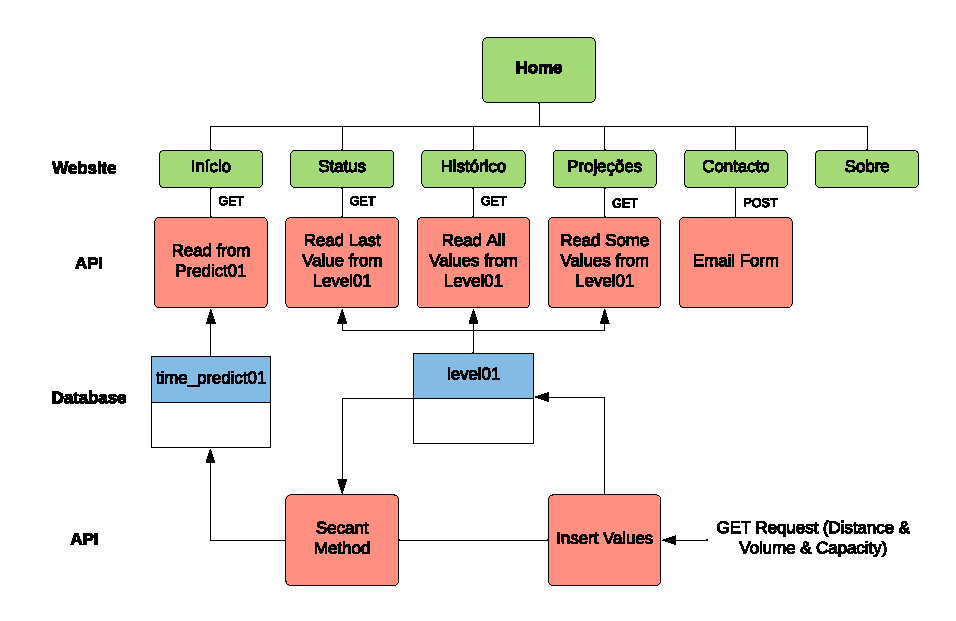
\includegraphics[scale=0.95]{images/Development/web_database/api_flowchart.pdf}
    \caption{Website structure diagram.}
    \label{fig:websiteDiagram}
\end{figure}

The communications are done by using \gls{HTTP} protocols, mostly through the GET and POST methods. It allows a large number of clients to access the platform simultaneously and, moreover, as the \gls{HTTP} supports the content negotiation, the client and servers can negotiate the desired format for a given resource, permitting the server to provide the same \gls{URL} in different formats, like \gls{JSON}, as approached by the Section~\ref{section:clienteSide}. These features increase the efficiency, flexibility and integration of the system.

The JavaScript is embedded inside of the \textit{main} element of the web document, where it will be located some features about the website \ref{subsection:features}. As the information is being dynamically updated, the consumer may have access of the last level measurement through the \gls{DHTML} document, by which provides a lot of benefits, as preview talked in Section~\ref{section:clienteSide}. 


\subsection{Web Application Features}\label{subsection:features}

In this Subsection, it is explored some features about the Web application relative to the data acquired from the measurements. It is important to highlight that, all the graphs were developed using Google Chart \gls{API}, which is a powerful free service that creates graphical charts from user-supplied data.


\subsubsection{Início}

In \textit{Início} (Start), the client might check the actual capacity of the reservoir and the status in case the system is unloading or loaded/loading. If the system is unloading, it will calculate the time remaining for the reservoir to drain out and, it will automatically show the date and time the reservoir will be totally empty. On the other side, if the system is already loaded or loading, it will only shows the actual capacity, as there is no date to estimate of when the reservoir will be empty (see Figure~\ref{fig:estimate}).

\begin{figure}[h!]
    \centering
    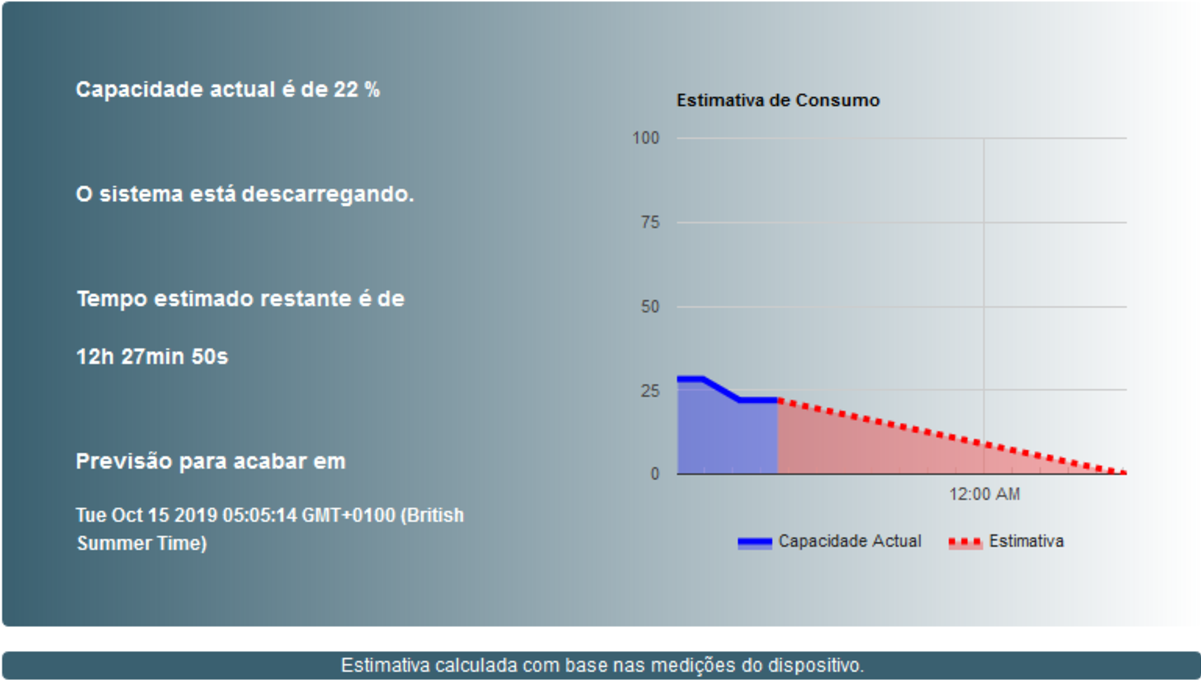
\includegraphics[scale=0.65]{images/Development/web_database/inicio1.pdf}
    \caption{Informative web page about the estimate graph of when the reservoir will be empty.}
    \label{fig:estimate}
\end{figure}

This calculus is possible by using a numerical solution for root-finding called secant method. As approached by \cite{GIFLAT:2013}, the method uses two points in neighborhood of the solution to determine a new estimate value. Therefore, it is possible to implement it by using a \gls{PHP} \gls{API}, where a new estimate value of the solution \begin{math}x_{i+1}\end{math} is determined from the previous two solutions \begin{math}x_i\end{math} and \begin{math}x_{i-1}\end{math}.

\begin{equation}\label{eq:secantMethod}
    x_{i+1}=x_i - \frac{f(x_i)(x_{i-1}-x_i)}{f(x_{i-1})-f(x_i)}
\end{equation}

The algorithm from the Equation~\ref{eq:secantMethod} was applied in the \gls{API} called Secant Method, as seen in Figure~\ref{fig:websiteDiagram}. It is responsible for reading the new information from the level01 table, process the data and stores the estimate date and time values in time\_predict01 table. Thus, the information is requested through \gls{AJAX} technique.


\subsubsection{Status}

In \textit{Status} page, as shown in Figure~\ref{fig:statusLayout}, the customer has the access to the last measurement values. It is a simple interface responsible for dynamically displaying the distance, volume, capacity and date and time values. The \gls{PHP} \gls{API} liable to provide the information for this Web page, only read the last value of the level01 table. Thereby, the server's response becomes much more responsive due the short length's size of the \gls{JSON} string.

\begin{figure}[h!]
    \centering
    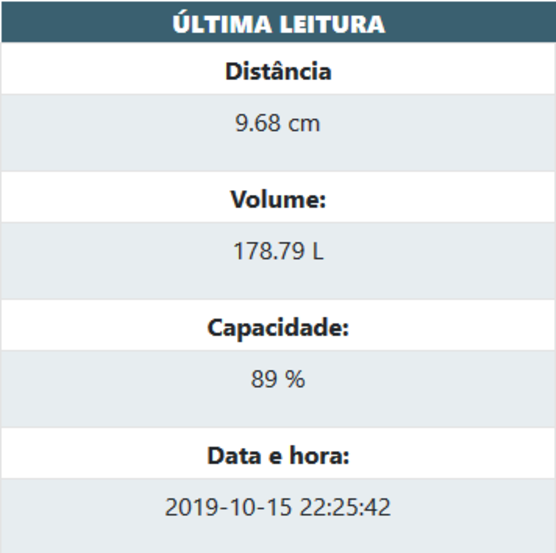
\includegraphics[scale=0.65]{images/Development/web_database/status1.pdf}
    \caption{Status layout.}
    \label{fig:statusLayout}
\end{figure}


\subsubsection{Histórico}

Already for the \textit{Histórico} (Historical), it was used the Bootstrap framework, which is an free and open source toolkit directed at responsive, mobile front-end web development that allows the client to navigate through the whole database content, permitting the user to sort and search all the information from the database however they want. 

Although this feature brings a lot of functionalities for the Web document, the \gls{API} responsible for that, needs to read all the information from the database at once, which makes the \gls{JSON} string, from the server's response, to be excessively large when the table has a large number of rows. Therefore, it can not be dynamically updated. The resulting interface can be seen in Figure~\ref{fig:historicTable}.

\begin{figure}[h!]
    \centering
    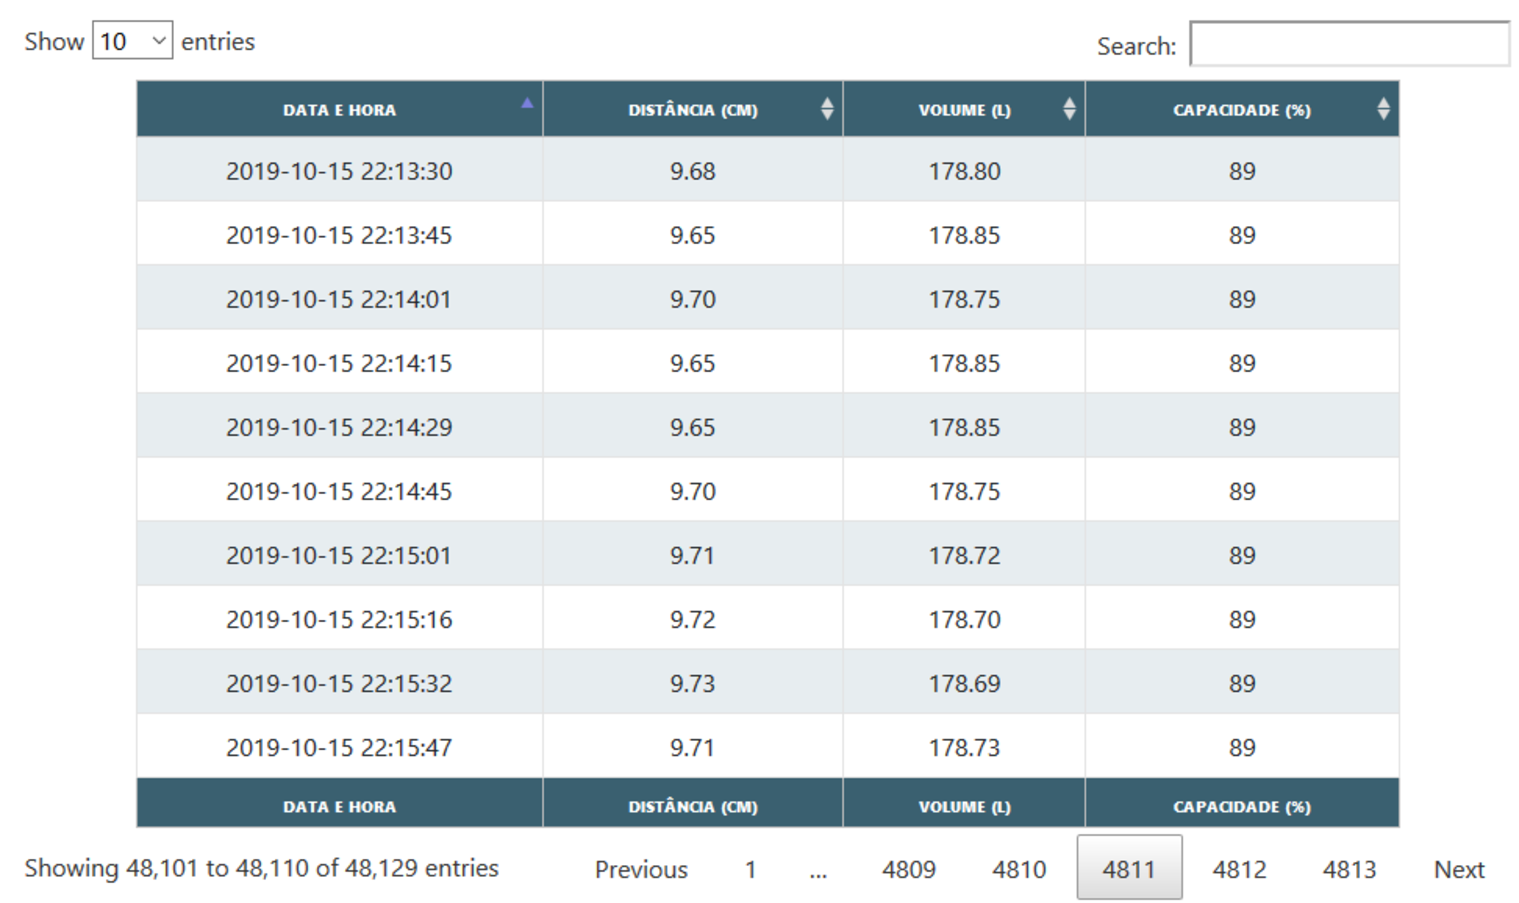
\includegraphics[scale=0.6]{images/Development/web_database/historico1.pdf}
    \caption{Historical table layout design and functionalities.}
    \label{fig:historicTable}
\end{figure}


\subsubsection{Projeções}

Taking a close look at \textit{Projeções} (Projections) page, it is responsible for showing the client a graph overview about the consumption of the reservoir's content. The Google Chart \gls{API} will read the last measurements from the device, this value can be configured by changing how much information the customer prefers, through the \gls{PHP} \gls{API} named \textit{Read Some Values from Level01}, shown in Figure~\ref{fig:websiteDiagram}. Although this value might be configured, it is not recommended to use a higher number as set in default, which is pre-configured for showing the last 500 measurements, due to the fact the Web page is being continuously updated via \gls{AJAX}, and it may overload the browser's cache memory, making it necessary to restart the browser in the course of time (see Figure~\ref{fig:projections}).

\begin{figure}[h!]
    \centering
    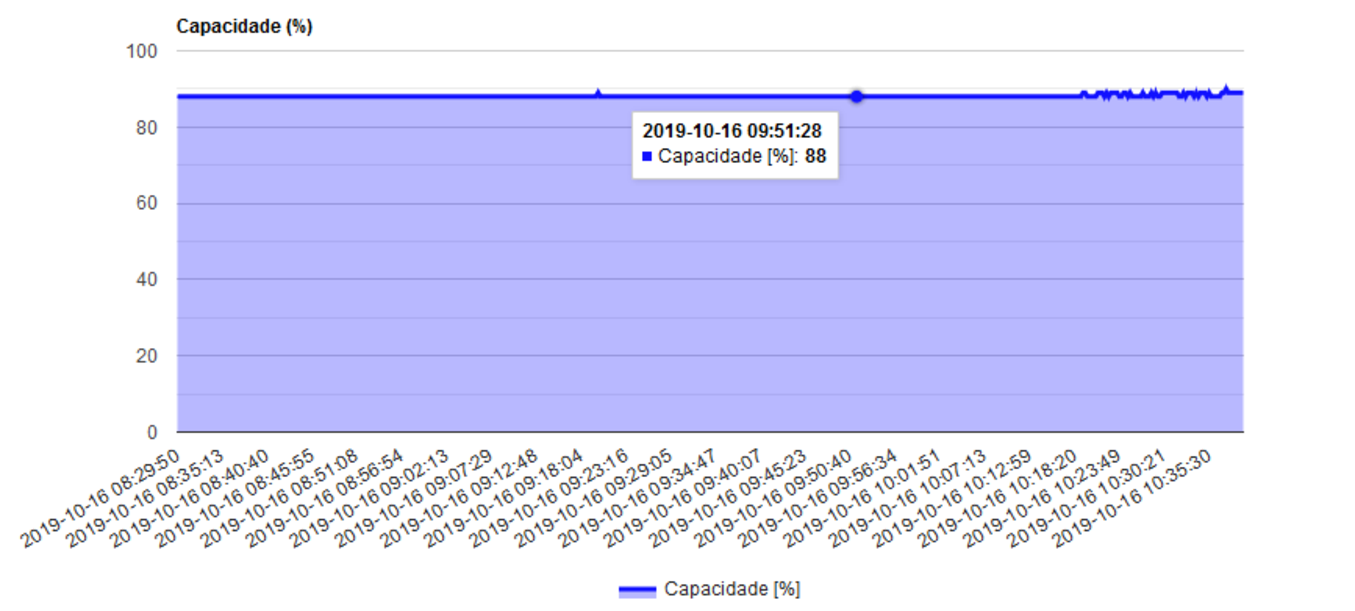
\includegraphics[scale=0.6]{images/Development/web_database/projecoes1.pdf}
    \caption{Graph design overview.}
    \label{fig:projections}
\end{figure}


\subsubsection{Contacto}

The last feature from the website is the \textit{Contacto} or Contact form, this feature allows the consumer to get in touch with the technicians, by sending to an pre-configured email address the description of the problem. It is a basic contact form that uses the POST method to request the \gls{API} to send an email using a local \textit{sendmail program}, through the \gls{PHP} function \textit{mail()}.

This feature is an integral part of any project or business, which allows a responsiveness and well-planned communication between the client and the system's responsible. The contact form layout can be seen in Figure~\ref{fig:contactForm}. 

\begin{figure}[h!]
    \centering
    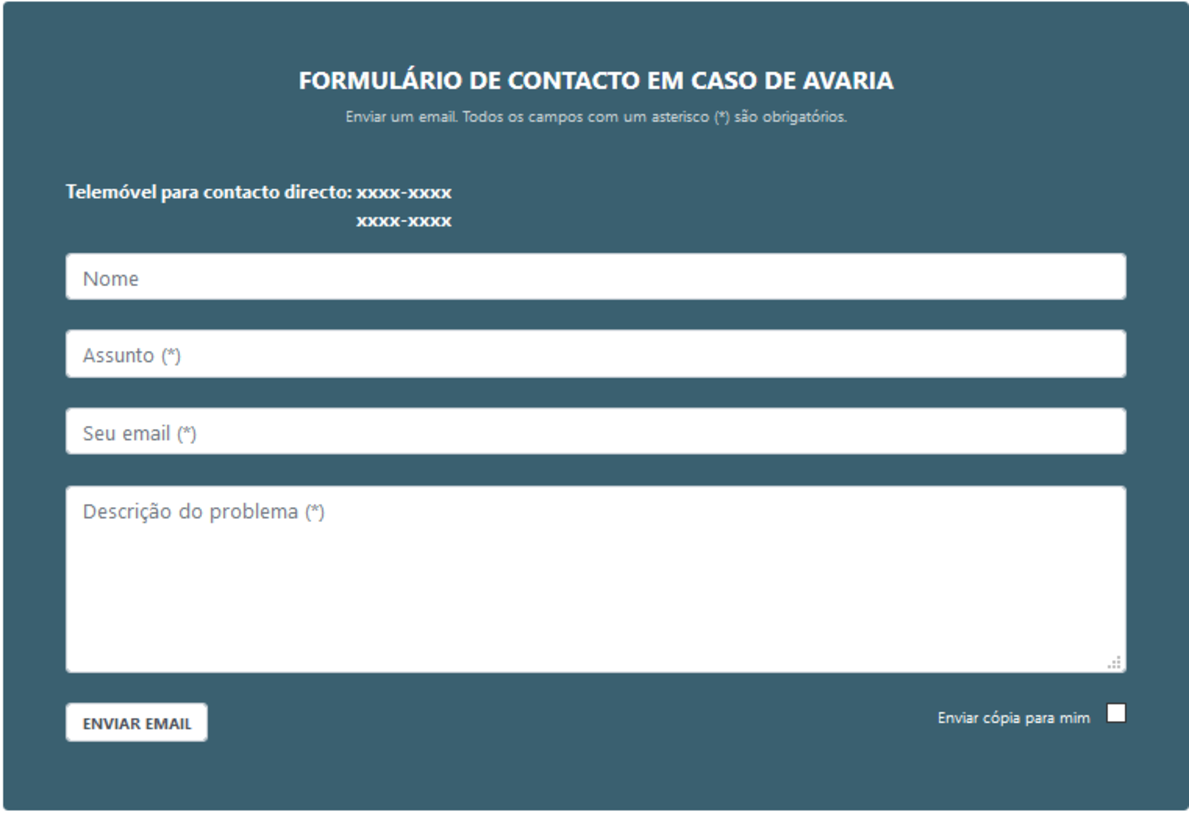
\includegraphics[scale=0.5]{images/Development/web_database/contacto1.pdf}
    \caption{Contact form layout design.}
    \label{fig:contactForm}
\end{figure}


\subsubsection{Sobre}

Lastly, in \textit{Sobre} (About) page, it is presented just a static \gls{HTML} text that provides, for the client, some basic information about the project.

\subsubsection{Website Address}

The website developed can be found by accessing the following \gls{URL}: \url{https://scmb-esp32.000webhostapp.com/application/index.php}.

It is important to point out that, due to the web technologies used here, the website content may not appear correctly for everyone, as it will depends about the hardware characteristics that is being used by the user. The browser version where the website was developed is based on \textit{Firefox version 69.0.3 (64-bit)}.